\documentclass[sigconf,anonymous]{acmart}

\title{VESPER: A High-Fidelity Smart Home Simulation Platform with
Firmware-in-the-Loop and LLM-Driven Activity Generation}
\author{Anonymous Author(s)}
\affiliation{%
  \institution{Anonymous Institution}
  \country{United States}
}

\setcopyright{none}
\settopmatter{printacmref=false}
\acmDOI{}\acmISBN{}\acmPrice{}

\usepackage{booktabs}
\usepackage{siunitx}
\sisetup{round-mode=places,round-precision=3}
\usepackage{graphicx}
\usepackage{subcaption}
\usepackage{microtype}
\usepackage{enumitem}
\usepackage{hyperref}
\usepackage{cleveref}
\usepackage{amsmath,mathtools}
\let\Bbbk\relax
\usepackage{amssymb}
\usepackage{listings}
\usepackage{xcolor}

% Define JSON language for listings (not built-in)
\lstdefinelanguage{json}{
  basicstyle=\ttfamily\footnotesize,
  string=[s]{"}{"},
  stringstyle=\color{blue!70!black},
  comment=[l]{//},
  morecomment=[s]{/*}{*/},
  literate=
    *{:}{{{\color{black!70}{:}}}}{1}
     {,}{{{\color{black!70}{,}}}}{1}
     {\{}{{{\color{black!70}{\{}}}}{1}
     {\}}{{{\color{black!70}{\}}}}}{1}
     {[}{{{\color{black!70}{[}}}}{1}
     {]}{{{\color{black!70}{]}}}}{1},
}
\usepackage{tikz}
\usepackage{pgfplots}
\pgfplotsset{compat=1.18}
\usetikzlibrary{shapes.symbols,shapes.geometric,positioning,arrows.meta,decorations.pathreplacing,calc}
\usepackage{colortbl}
\usepackage{pifont}

% Define colors for architecture diagram
\definecolor{habitatcolor}{RGB}{70,130,180}
\definecolor{firmwarecolor}{RGB}{220,120,50}
\definecolor{llmcolor}{RGB}{100,180,100}
\definecolor{cloudcolor}{RGB}{150,100,200}
\definecolor{buscolor}{RGB}{255,200,100}

\newcommand{\sys}{\textsc{VESPER}}

\lstset{
  basicstyle=\ttfamily\small,
  keywordstyle=\color{blue},
  commentstyle=\color{gray},
  breaklines=true,
  frame=single,
}

\settopmatter{printacmref=false, printccs=false, printfolios=false}
\renewcommand\footnotetextcopyrightpermission[1]{}
\setcopyright{none}
\acmConference{}{}{}
\acmBooktitle{}

\begin{document}

\begin{abstract}
Testing and evaluating IoT systems at scale remains a fundamental
challenge: physical testbeds are expensive, difficult to reproduce,
and limited in scope, while existing simulators lack the fidelity
needed for realistic device firmware behavior and human activity
patterns.  We present \sys{}, a high-fidelity smart home simulation
platform that combines three innovations:
(1)~\emph{firmware-in-the-loop} emulation via QEMU-based ARM
containers running real device firmware alongside a 3D household
simulation (Habitat~3.0);
(2)~\emph{LLM-driven humanoid activity generation} that produces
diverse daily schedules conditioned on structured
occupant personas; and
(3)~\emph{bi-directional cloud synchronization} with Samsung
SmartThings for Sim2Real validation.
Our evaluation across five research questions and a large-scale
autonomous study (28~HSSD scenes, 7~simulated days each,
88.0~hours wall-clock time) demonstrates
that \sys{}-generated activity patterns exhibit moderate distributional
similarity to real-world datasets (CASAS, ARAS) with a mean
JS~divergence of~0.218, outperforming a learned Markov baseline
on diverse multi-occupant homes (50--62\% lower JS on ARAS).
The platform scales to 200 concurrent devices at over
10{,}000~events/s with sub-36\% CPU utilization and achieves
microsecond-scale event-bus dispatch (P99 $= 7$\,$\mu$s).
A security assessment of 982~attacks across five suites---firmware,
network, phantom-delay, malicious SmartApp, and ESP32 buffer
overflow---against six device types yields a 67.4\% exploit rate
with a mean CVSS~3.1 score of~8.1, validated against 24~real-world
CVEs and covering 7 of 10 OWASP IoT Top~10 categories.
Packet-level traffic analysis---validated by \texttt{tshark}
pcap captures independently verifiable with Wireshark---records
154{,}151~TCP segments (12.1\,MB) across 980~attack executions
in 28~scenes, confirming that all attack traffic traverses the
real Docker bridge network.
An enriched Sim2Real transfer analysis achieves 0.813~accuracy
on ARAS-A using 119-dimensional feature representations.
The autonomous evaluation achieves 94.9\%
navigation success across 3{,}580~trials, generates
47{,}207 firmware-triggered SmartThings cloud updates with zero data
loss, and produces 4{,}307~LLM-generated tasks using GPT-OSS~20B.
All results pass an 8-point reproducibility check against raw data.
To our knowledge, \sys{} is the first platform to unify embodied
AI simulation, real firmware execution, and cloud-connected IoT
in a single reproducible framework.
\end{abstract}

\keywords{Smart Home Simulation, IoT Testing, Firmware-in-the-Loop,
LLM Activity Generation, Habitat 3.0, Digital Twin}

\maketitle

% ---- Section files ----
\section{Introduction}\label{sec:intro}

The Internet of Things (IoT) is transforming residential environments
into complex cyber-physical systems.  A modern smart home may contain
dozens of heterogeneous devices---sensors, actuators, voice assistants,
and hub controllers---whose interactions with human occupants produce
rich, privacy-sensitive data streams.  Researchers studying smart home
security~\cite{iot-security-survey}, energy optimization~\cite{iot-energy-survey}, and activity
recognition~\cite{har-survey} all share a common bottleneck: the need for
\emph{realistic, large-scale, and reproducible} testbeds.

Physical smart home testbeds~\cite{iot-testbed-survey} are expensive to construct,
difficult to instrument, and inherently limited to a single floor plan
and occupant population.  Software-only simulators such as
OpenHAB-Sim~\cite{openhab-sim} and IoTSim~\cite{iotsim} improve reproducibility but
sacrifice fidelity: they model devices as stateless message endpoints,
ignore firmware-level behavior, and generate occupant activity through
simple Markov chains that fail to capture the contextual richness of
real daily routines.

We present \sys{} (\textbf{V}irtual \textbf{E}nvironment for
\textbf{S}mart-home \textbf{P}latform \textbf{E}valuation and
\textbf{R}esearch), a simulation platform that addresses these
limitations through three tightly integrated innovations:

\begin{enumerate}[leftmargin=*]
  \item \textbf{Firmware-in-the-loop emulation.}
    \sys{} runs real ARM device firmware inside QEMU containers
    managed by Docker, enabling bit-accurate execution of sensor
    sampling loops, interrupt handlers, and communication stacks
    (UART-over-TCP, MQTT).  Each virtual device exposes a network
    interface matching its physical counterpart's protocol.

  \item \textbf{LLM-driven activity generation.}
    Rather than relying on hand-crafted Markov models, \sys{} uses
    large language models (via LMStudio) to generate daily activity
    schedules conditioned on detailed occupant personas (age,
    occupation, mobility constraints, lifestyle preferences).  This
    produces statistically diverse yet contextually coherent
    behavioral patterns.

  \item \textbf{Bi-directional cloud synchronization.}
    \sys{} implements the Samsung SmartThings Schema Connector
    protocol, allowing simulated devices to appear as first-class
    citizens in a real SmartThings account.  State changes flow
    in both directions, enabling Sim2Real validation of automations,
    routines, and third-party integrations.
\end{enumerate}

These components are unified within Meta's Habitat~3.0 embodied AI
framework, which provides physics-accurate 3D scene rendering,
humanoid navigation, and object interaction.  A central event bus
coordinates real-time data flow among all subsystems at
sub-millisecond latency.

\paragraph{Contributions.}
\begin{itemize}[leftmargin=*]
  \item The design and implementation of \sys{}, a smart home
    simulation platform that, to our knowledge, is the first to
    combine embodied 3D simulation, firmware-in-the-loop emulation,
    and cloud-connected IoT in a single reproducible framework.
  \item An LLM-based activity generation pipeline with a library of
    10~diverse personas, producing schedules whose distributions
    show moderate alignment with real-world datasets (CASAS, ARAS)
    with a mean JS divergence of~0.218 across five reference homes,
    outperforming a learned Markov baseline on diverse multi-occupant
    environments.
  \item A comprehensive evaluation across five research questions,
    demonstrating fidelity (with baseline comparison), scalability,
    latency, Sim2Real transfer potential (0.813~accuracy on ARAS-A
    via enriched 119-feature representations), and security
    assessment capability (validated against 24~real-world CVEs
    covering 7 of 10 OWASP IoT Top~10 categories).
  \item A large-scale autonomous evaluation across 28~HSSD scenes
    over 7~simulated days each (88.0~hours wall-clock), validating
    end-to-end reliability with 94.9\% navigation success,
    47{,}207~firmware-triggered cloud updates, and
    4{,}307~LLM-generated tasks.
  \item A security testing framework comprising 36~unique attacks
    across five suites (firmware, network, phantom-delay, malicious
    SmartApp, ESP32 buffer overflow) with automated CVSS~3.1 scoring
    and MITRE ATT\&CK mapping, yielding the first IoT security
    evaluation integrated within an embodied simulation platform.
    Packet-level traffic analysis---validated by \texttt{tshark}
    pcap captures (154{,}151~TCP segments, 12.1\,MB global capture,
    736~individual pcap files)---confirms that all attack traffic
    traverses the real Docker bridge network and is independently
    verifiable with Wireshark.
  \item An open-source release of the platform, evaluation framework,
    and all experiment configurations for full reproducibility.
\end{itemize}

\section{Background}\label{sec:background}

\subsection{Smart Home Simulation}

Simulating smart home environments requires modeling three
interdependent domains: the \emph{physical space} (rooms, furniture,
appliances), the \emph{occupant behavior} (movement, activities,
routines), and the \emph{device ecosystem} (sensors, actuators,
communication protocols, cloud services).  Existing tools address
these in isolation.

\textbf{3D Embodied Simulation.}
Habitat~\cite{habitat19iccv,habitat2,habitat3}, AI2-THOR~\cite{ai2thor},
and iGibson~\cite{igibson} provide photorealistic 3D environments with
physics engines, but focus on embodied AI navigation tasks rather
than IoT device modeling.  Habitat~3.0 introduced humanoid avatars
with realistic motion and multi-agent coordination, making it
suitable as a foundation for occupant simulation.

\textbf{IoT Testbeds and Simulators.}
IoTSim~\cite{iotsim}, FIESTA-IoT~\cite{fiesta-iot}, and SWoTSuite~\cite{swotsuite} model
device networks but lack 3D spatial grounding.  They represent devices
as abstract message endpoints, missing firmware-level behaviors such as
sensor drift, interrupt timing, and flash-storage wear.

\textbf{Activity Generation.}
Traditional approaches use Markov chains~\cite{markov-activity}, stochastic Petri
nets~\cite{petri-net-activity}, or agent-based models~\cite{abm-activity} to generate occupant
activities.  These methods require extensive manual parameterization
and struggle to produce the contextual variety observed in real
households with diverse occupant demographics.

\subsection{Firmware-in-the-Loop Testing}

Firmware-in-the-loop (FIL) testing runs actual device firmware on
emulated hardware to catch bugs that unit tests and hardware-in-the-loop
setups miss.  QEMU~\cite{qemu} provides full-system ARM emulation and has
been used for IoT firmware analysis~\cite{firmadyne,avatar}.  \sys{}
packages QEMU instances in Docker containers, each running a compiled
ARM binary with simulated GPIO, UART, and network peripherals.

\subsection{LLMs for Behavioral Modeling}

Recent work has explored LLMs as world models~\cite{llm-world-model} and behavior
planners~\cite{llm-planner}.  Park et al.~\cite{generative-agents} demonstrated
that LLM-driven agents can produce believable daily routines in a
virtual town.  \sys{} adapts this insight to the smart home domain:
instead of open-ended sandbox behavior, we use structured prompts to
generate \emph{activity schedules}---timestamped sequences of
activities with room assignments and device interactions---that can be
validated against real-world activity datasets.

\subsection{SmartThings Ecosystem}

Samsung SmartThings is a leading IoT cloud platform supporting
hundreds of device types via its Schema Connector and Device
Profiles.  The Schema Connector protocol defines a webhook-based
lifecycle (discovery, state refresh, command handling) through which
third-party devices integrate with the SmartThings app.  \sys{}'s
bridge implements this protocol, allowing simulated devices to appear
alongside real hardware in a user's SmartThings account.

\section{System Design}\label{sec:design}

\begin{figure*}[t]
  \centering
  % If the figure is too tall, switch to height=0.33\textheight (or similar).
  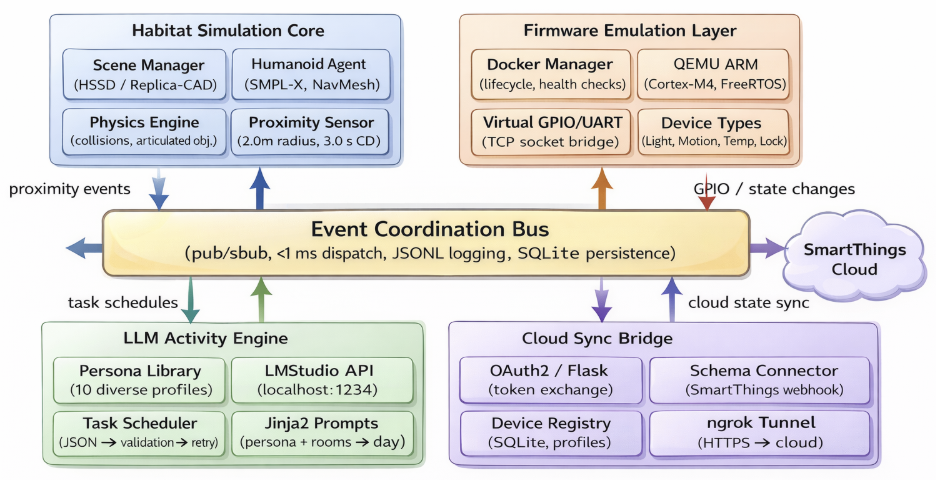
\includegraphics[width=\textwidth]{figures/architecture.png}
  \caption{Architecture of \sys{}. Seven functional layers communicate through a central publish-subscribe event coordination bus. Double-headed arrows denote bi-directional real-time data flow. The Cloud Sync Bridge connects to Samsung SmartThings via an ngrok HTTPS tunnel.}
  \label{fig:architecture}
\end{figure*}



\sys{} comprises seven layers (\Cref{fig:architecture}):
the \emph{Habitat Simulation Core}, the \emph{Firmware Emulation
Layer}, the \emph{LLM Activity Engine}, the \emph{Cloud Sync
Bridge}, the \emph{Event Coordination Bus}, the \emph{Simulated
Home Network}, and the \emph{Security Testing Layer}.

\subsection{Habitat Simulation Core}

The simulation core wraps Meta Habitat~3.0 to provide:
\begin{itemize}[leftmargin=*]
  \item \textbf{Scene management.}  HSSD~\cite{hssd} and Replica-CAD scene
    datasets supply photorealistic room layouts with furniture and
    appliance meshes.
  \item \textbf{Humanoid agents.}  SMPL-X parametric humanoid models
    navigate rooms, interact with objects (e.g., opening doors,
    picking up items), and trigger device proximity events.
  \item \textbf{Physics engine.}  Bullet physics provides collision
    detection and object manipulation, enabling realistic interactions
    between humanoids and IoT-instrumented objects.
\end{itemize}

\subsection{Firmware Emulation Layer}\label{sec:firmware-layer}

Each simulated IoT device is backed by a Docker container running
QEMU~10.2 in ARM system-emulation mode targeting the
\textbf{LM3S6965EVB} evaluation board (ARM Cortex-M3, Thumb ISA).
Unlike prior IoT testbeds that use host-side mocks, \sys{} executes
\emph{real} bare-metal firmware---compiled from C with
\texttt{arm-none-eabi-gcc}---inside QEMU's instruction-accurate
emulator, preserving interrupt semantics, register state, and
memory layout (though not cycle-level timing).

\paragraph{Per-Device Firmware Variants.}
We provide six firmware images, each implementing a device-specific
command set and sensor model:
\begin{enumerate}[leftmargin=*]
  \item \textbf{Smart Light} --- PWM brightness (0--100\%), color
    temperature (2\,700--6\,500\,K), on/off/toggle.
  \item \textbf{Motion Sensor} --- PIR interrupt with configurable
    sensitivity (1--10) and cooldown timer.
  \item \textbf{Temperature Sensor} --- ADC sampling at 1\,Hz with
    Kalman filtering and threshold alerts.
  \item \textbf{Humidity Sensor} --- relative-humidity and
    temperature combo sensor with calibration.
  \item \textbf{Door Sensor} --- magnetic contact with
    open/closed state and tamper detection.
  \item \textbf{Smart Plug} --- relay-driven outlet with power
    metering (watts) and scheduling.
\end{enumerate}
All six variants share a common skeleton (ISR vector table, UART
driver, command dispatcher) and are compiled with identical flags
(\texttt{-mcpu=cortex-m3 -mthumb -Os -nostartfiles -nostdlib}).
A custom linker script places the ISR vector in \texttt{.isr\_vector}
and allocates 64\,KB flash / 20\,KB SRAM, matching the physical
LM3S6965 memory map.

\paragraph{UART Protocol.}
Firmware communicates with the host through UART0 mapped to a TCP
socket (\texttt{-serial tcp::15000,server,nowait}).  The protocol
uses newline-terminated ASCII commands:
\begin{itemize}[leftmargin=*]
  \item \texttt{IDENTIFY} / \texttt{ID} --- returns device type,
    capabilities, firmware version, and unique ID.
  \item \texttt{ON}, \texttt{OFF}, \texttt{TOGGLE},
    \texttt{STATUS}, \texttt{GET\_ALL} --- power and state control.
  \item \texttt{SET\_ID}, \texttt{AUTH} --- device provisioning and
    token-based authentication.
  \item \texttt{FW\_UPDATE:<hex>}, \texttt{FW\_APPLY} --- over-the-air
    firmware update (intentionally unauthenticated).
  \item \texttt{DEBUG\_DUMP} --- diagnostic command that leaks
    internal buffers (intentional vulnerability).
  \item Device-specific commands (e.g., \texttt{SET\_BRIGHTNESS},
    \texttt{SET\_SENSITIVITY}, \texttt{CALIBRATE}).
\end{itemize}

\paragraph{Intentional Vulnerability Model.}
Each firmware embeds three classes of vulnerability by design:
(i)~a \emph{buffer overflow} in the firmware-update handler, where
the 128-byte \texttt{fw\_update\_buf} accepts data without bounds
checking;
(ii)~\emph{missing authentication}, as all commands execute without
verifying the \texttt{AUTH} token; and
(iii)~\emph{information disclosure} via the \texttt{DEBUG\_DUMP}
command, which returns the cleartext auth token and firmware buffer
contents.
These mirror CVE patterns commonly found in commodity IoT
devices~\cite{owasp-iot-top10} and serve as ground-truth targets
for the security evaluation (\Cref{sec:eval-rq5}).

\paragraph{Firmware--Simulation Coupling.}
The firmware layer supports two operational modes through the same
UART-over-TCP interface:
(i)~\emph{normal operation}, where humanoid proximity in the 3D
scene triggers GPIO interrupts that drive realistic device behavior;
and
(ii)~\emph{security testing}, where attack scripts inject malicious
commands directly to the firmware to assess vulnerability resilience.
In normal mode, when a humanoid agent approaches a device in the 3D
scene, the event bus publishes a proximity event.  The corresponding
firmware container receives the event as a GPIO interrupt, executes
its real ISR handler, and emits a state-change message
(e.g., \texttt{light:on}) back through the bus.  In security mode,
the same firmware processes crafted payloads from the attack
framework, enabling vulnerability discovery without requiring
3D simulation overhead.  This dual-mode design makes \sys{} suitable
for both behavioral fidelity studies (RQ1--RQ4) and security
assessment (RQ5).

\subsection{LLM Activity Engine}

\paragraph{Persona model.}
A \emph{persona} is a structured description of a household occupant:
age, occupation, mobility level, wake/sleep times, and lifestyle
preferences.  We provide a library of 10~diverse personas
(\Cref{tab:personas}) covering young professionals, retirees, shift
workers, students, and individuals with mobility constraints.

\begin{table}[t]
  \centering
  \caption{Persona library used for LLM-driven schedule generation.
  Each persona defines demographic and lifestyle attributes that
  condition the LLM prompt.}
  \label{tab:personas}
  \small
  \begin{tabular}{l l l l}
    \toprule
    {Persona} & {Age} & {Occupation} & {Wake/Sleep} \\
    \midrule
    Alex   & 28 & Software Engineer   & 07:00 / 23:00 \\
    Maria  & 67 & Retired Teacher     & 06:00 / 21:30 \\
    James  & 35 & Shift Worker        & 14:00 / 04:00 \\
    Priya  & 22 & Graduate Student    & 08:30 / 01:00 \\
    Carlos & 45 & Remote Manager      & 06:30 / 22:30 \\
    Yuki   & 31 & Freelance Artist    & 09:00 / 00:30 \\
    Robert & 72 & Retired (mobility)  & 05:30 / 20:00 \\
    Sarah  & 40 & Nurse (night shift) & 16:00 / 06:00 \\
    David  & 19 & College Student     & 10:00 / 02:00 \\
    Lin    & 55 & Restaurant Owner    & 04:30 / 21:00 \\
    \bottomrule
  \end{tabular}
\end{table}


\paragraph{Schedule generation.}
Given a persona and a day type (weekday/weekend), the Activity Engine
prompts a local LLM (served by LMStudio) to produce a JSON-formatted
daily schedule:
\begin{lstlisting}[language=json,basicstyle=\ttfamily\footnotesize]
[
  {"time": "06:30", "activity": "Wake up",
   "room": "Bedroom", "duration": 15,
   "devices": ["smart_light", "thermostat"]},
  ...
]
\end{lstlisting}
A validation layer parses the JSON, resolves room names against the
loaded scene, and fills any missing fields with defaults.  Invalid
schedules trigger a retry with explicit error feedback in the prompt.

\begin{figure}[t]
  \centering
  \small
  \setlength{\tabcolsep}{3pt}
  \begin{tabular}{@{}r l l l@{}}
    \toprule
    \textbf{Time} & \textbf{Activity} & \textbf{Room} & \textbf{Devices} \\
    \midrule
    \rowcolor{blue!5}
    06:30 & Wake up          & Bedroom   & \texttt{light} \\
    06:45 & Morning hygiene  & Bathroom  & \texttt{light} \\
    07:15 & Breakfast        & Kitchen   & \texttt{light, temp} \\
    \rowcolor{blue!5}
    08:00 & Work session     & Office    & \texttt{light} \\
    12:00 & Lunch prep       & Kitchen   & \texttt{light, temp} \\
    12:30 & Lunch            & Dining    & \texttt{light} \\
    \rowcolor{blue!5}
    13:00 & Work session     & Office    & \texttt{light} \\
    15:30 & Coffee break     & Kitchen   & \texttt{light} \\
    17:00 & Exercise         & Living    & \texttt{motion} \\
    \rowcolor{blue!5}
    18:00 & Dinner prep      & Kitchen   & \texttt{light, temp} \\
    19:00 & Dinner           & Dining    & \texttt{light} \\
    20:00 & Evening reading  & Living    & \texttt{light} \\
    \rowcolor{blue!5}
    21:30 & Wind down        & Bedroom   & \texttt{light} \\
    22:00 & Sleep            & Bedroom   & \texttt{light} \\
    \bottomrule
  \end{tabular}
  \caption{Example LLM-generated daily schedule for the ``Alex''
  persona (28-year-old software engineer, weekday).  The schedule
  shows realistic circadian structure, room transitions, and
  device interactions that trigger firmware events.}
  \label{fig:schedule-example}
\end{figure}


\Cref{fig:schedule-example} shows an example generated schedule,
illustrating the realistic room transitions and device interactions.

\subsection{Cloud Sync Bridge}

The Sync Bridge implements the SmartThings Schema Connector
protocol~\cite{smartthings-schema}.  It handles:
\begin{itemize}[leftmargin=*]
  \item \textbf{OAuth2 token exchange.}  A local Flask server
    completes the SmartThings callback flow, exchanging authorization
    codes for access and refresh tokens.
  \item \textbf{Device discovery.}  Simulated devices are registered
    in a SQLite \emph{Device Registry} with SmartThings-compatible
    device profiles (capabilities, categories).
  \item \textbf{State sync.}  A background coroutine pushes state
    updates to SmartThings via the State Callback URL; incoming
    commands from the SmartThings app or automations are dispatched
    to the corresponding firmware container.
\end{itemize}

\subsection{Event Coordination Bus}

A lightweight publish-subscribe event bus connects all layers with
sub-millisecond dispatch.  Events carry a typed payload
(\texttt{device\_state}, \texttt{proximity}, \texttt{task\_update},
\texttt{firmware\_event}), a nanosecond-precision timestamp, and a
source identifier.  The bus also provides:
\begin{itemize}[leftmargin=*]
  \item \textbf{History buffer.}  A configurable ring buffer retains
    recent events for temporal queries.
  \item \textbf{JSONL logging.}  All events are persisted to a
    structured log for post-hoc analysis.
  \item \textbf{SQLite task database.}  Completed tasks are stored
    with category, room, duration, and outcome metadata for
    statistical analysis.
\end{itemize}

\subsection{Simulated Home Network}\label{sec:home-network}

To evaluate network-level attacks in a controlled environment,
\sys{} instantiates a \emph{Simulated Home Network} that replicates
the topology and protocols of a typical residential IoT deployment.

\paragraph{Network Topology.}
The network supports four Docker driver modes---\emph{bridge}
(default), \emph{macvlan}, \emph{ipvlan}, and \emph{host}---selected
via a single \texttt{NetworkMode} configuration parameter.
The default bridge network (\texttt{vesper-home-network},
\texttt{172.20.0.0/24}) interconnects all device containers, a
central MQTT broker (\texttt{172.20.0.2}), and the host-side
attack runner.  Each device is assigned a static IP starting at
\texttt{172.20.0.10}, with configurable link parameters: base
latency 5.0\,ms $\pm$ 2.0\,ms jitter, 100\,Mbps bandwidth, and
adjustable packet-loss ratio.  The macvlan mode attaches containers
directly to a physical network interface (auto-detected or
user-specified), enabling Wireshark capture of real traffic frames
on the host NIC---useful for protocol debugging and forensic analysis.

\paragraph{Protocol Simulators.}
In addition to TCP/MQTT, the simulated network includes pluggable
protocol simulators for Zigbee, Z-Wave, and Bluetooth Low Energy
(BLE).  Each simulator models basic message routing, device
registration, and network-key generation at the application layer
(not full RF-level framing).  This enables simulated protocol-layer
attacks (e.g., Zigbee replay, key extraction) within the Docker
network, though attacks requiring physical-layer access (RF
jamming, deauthentication frames) are modeled conceptually
rather than executed on real wireless interfaces.

\paragraph{MQTT Broker.}
A lightweight text-based MQTT broker handles publish/subscribe for
device state updates using a hierarchical topic scheme
(\texttt{vesper/devices/<id>/state|events|commands}).
The broker supports wildcard subscriptions (\texttt{\#}, \texttt{+}),
retained messages, and optional username/password authentication.
By default, authentication is \emph{disabled}, replicating the
insecure default configurations found in many consumer IoT hubs.

\paragraph{Packet Capture.}
A dual-path capture architecture records all attack traffic for
post-hoc analysis.  In all network modes, an
\texttt{InstrumentedSocket} wrapper logs every TX/RX payload with
nanosecond timestamps at the application layer.  In addition,
\texttt{tshark} (Wireshark CLI) captures raw TCP segments on the
loopback interface via BPF filters, producing genuine
\texttt{.pcap} files independently verifiable with Wireshark or
\texttt{tcpdump}.
We validate this capture architecture in
\Cref{sec:eval-pcap}: a full 980-attack campaign across 28~scenes
yields 154{,}151~TCP segments (12.1\,MB) in
736~per-attack pcap files plus a global session capture
(\Cref{tab:traffic-analysis,tab:protocol-breakdown}).

\subsection{Security Testing Layer}\label{sec:security-layer}

\sys{} integrates a five-suite security testing framework that
evaluates firmware-level, network-level, protocol-level, cloud API,
and memory-safety vulnerabilities.

\paragraph{Firmware Attack Framework.}
The firmware attack suite comprises 18~attacks organized into
nine categories: buffer overflow, command injection, authentication
bypass, firmware update exploitation, information disclosure,
denial of service, state manipulation, replay, and protocol fuzzing.
Each attack communicates with the target firmware through the same
UART-over-TCP channel used by legitimate commands, ensuring that
attack traffic traverses the full emulation stack (QEMU interrupt
controller $\to$ ISR $\to$ UART driver $\to$ command parser).
Attacks are scored with CVSS~v3.1 base vectors and return structured
results including exploit evidence, impact assessment, and mitigation
recommendations.

\paragraph{Network Attack Framework.}
A complementary suite of 14~network-level attacks targets the
simulated home network across five attack suites: MQTT attacks
(eavesdropping, message injection, topic hijacking), TCP/IP attacks
(connection hijacking, man-in-the-middle, SYN flooding),
simulated protocol-specific attacks (Zigbee replay, key extraction,
protocol downgrade), infrastructure attacks (ARP spoofing on Docker
bridge; DNS poisoning and WiFi deauthentication modeled
conceptually), and traffic analysis attacks (simulated evil twin AP,
active traffic fingerprinting).

\paragraph{Malicious SmartApp (Suite~4).}
A rogue SmartApp attack targets the SmartThings Schema Connector
to exploit over-broad OAuth scopes (CWE-269, CWE-862, CVSS~8.8).
The attack probes the connector's HTTP endpoint, enumerates all
registered devices via a \texttt{discoveryRequest} without valid
credentials, steals the OAuth callback token through a
\texttt{stateRefreshRequest}, and injects arbitrary commands
(e.g., DISARM) via a forged \texttt{commandRequest}.
This demonstrates the risk of insufficient access control in
cloud-connected IoT integrations.

\paragraph{ESP32 Buffer Overflow (Suite~5).}
A stack buffer overflow attack targets the 128-byte command buffer
in the ESP32 firmware (CWE-120, CWE-787, CVSS~9.8).  The attack
constructs a 137-byte payload containing a 32-byte NOP sled
(Thumb-mode \texttt{0xBF00} instructions), a shellcode marker, and
a crafted return address (LR offset~132, targeting mid-SRAM at
\texttt{0x20000080}) that overwrites the saved link register on the
Cortex-M3 stack.  The exploit causes device crash/DoS, with the
potential for arbitrary code execution with a refined payload.

\paragraph{Published Attack Reproduction.}
To validate \sys{} as a research platform for IoT security,
we reproduce the \emph{Phantom-Delay Attack}~\cite{phantom-delay},
a protocol-level exploit targeting IoT timeout behaviors.
Fu~et~al.\ demonstrated that an attacker on the local network can
establish a transparent TCP proxy via ARP spoofing and selectively
delay device event messages for up to 40~minutes (Apple~HomeKit)
or 64~seconds (Ring~Security) without triggering device-offline
alerts.  The delayed events are still accepted by the hub,
enabling four attack variants: \emph{state-update delay}
(stale alerts), \emph{erroneous automation execution}
(trigger with wrong condition), \emph{routine invalidation}
(exceed cloud timeout threshold), and \emph{action reorder}
(swap command order).  Our implementation adapts all four variants
for \sys{}'s Docker bridge network, where the same UART-over-TCP
and MQTT channels used by legitimate firmware communication serve
as the attack surface (\Cref{sec:eval-phantom-delay}).

Together, the five suites comprise 36~unique attack implementations
covering 83\% of MITRE ATT\&CK for IoT tactics and all seven stages
of the IoT Cyber Kill Chain.

\section{Implementation}\label{sec:implementation}

\sys{} is implemented in approximately 15{,}000 lines of core
Python~3.9 (excluding tests, scripts, and evaluation tooling),
with ARM firmware written in bare-metal C ($\sim$1{,}600 lines across
six device variants).  We highlight key implementation
decisions below.

\subsection{3D Simulation}

We build on Habitat-Lab v0.3.0 with the Habitat-Sim renderer.
Scenes are loaded from the HSSD-Hab and Replica-CAD datasets.
Humanoid navigation uses the built-in shortest-path follower with a
custom task scheduler that dispatches activities from the LLM-generated
schedule.  Object interactions (pick, place, open, toggle) use
Habitat's rearrangement primitives.

\subsection{Firmware Containers}

Each device type has a corresponding Dockerfile that:
\begin{enumerate}
  \item Installs the QEMU ARM system emulator (v10.2).
  \item Copies the pre-compiled firmware ELF binary for the
    target device type.
  \item Exposes a TCP socket (default port~15\,000) for UART I/O.
  \item Launches QEMU with the LM3S6965EVB machine profile:\\
    \texttt{qemu-system-arm -machine lm3s6965evb}\\
    \texttt{-cpu cortex-m3 -nographic}\\
    \texttt{-kernel <device>.elf}\\
    \texttt{-serial tcp::15000,server,nowait}
\end{enumerate}
A Python \texttt{DeviceFirmwareManager} class wraps the Docker SDK to
create, start, stop, and remove containers.  Health checks ping the
TCP socket; unresponsive containers are restarted automatically.
A \texttt{DeviceType} enum with 28~name aliases (e.g., ``thermostat''
$\to$ \textsc{Temperature\_Sensor}, ``bulb'' $\to$
\textsc{Smart\_Light}) enables fuzzy device-type resolution from
natural-language scene descriptions.

\paragraph{Firmware Build System.}
All six firmware variants are compiled with a shared Makefile using
\texttt{arm-none-eabi-gcc} and the flags
\texttt{-mcpu=cortex-m3 -mthumb -Os -nostartfiles -nostdlib
-ffunction-sections -fdata-sections}.  A custom linker script
(\texttt{linker.ld}) maps the ISR vector table to flash address
\texttt{0x0000\_0000} and allocates 64\,KB flash and 20\,KB SRAM.
Each firmware image is approximately 300~lines of C implementing
the UART driver (PL011-compatible registers at \texttt{0x4000C000}),
command dispatcher, GPIO handlers, and device-specific sensor models.
The build produces both ELF (for QEMU) and raw binary outputs.

We provide reference firmware images for six device types:
\begin{itemize}[leftmargin=*]
  \item \textbf{Smart Light} --- PWM-controlled LED with on/off/dim,
    brightness (0--100\%), and color temperature
    (2\,700--6\,500\,K).
  \item \textbf{Motion Sensor} --- PIR interrupt with configurable
    sensitivity (1--10) and cooldown timer.
  \item \textbf{Temperature Sensor} --- ADC sampling at 1\,Hz with
    Kalman filtering and threshold alerts.
  \item \textbf{Humidity Sensor} --- combined RH\% and temperature
    monitoring with user-invocable calibration.
  \item \textbf{Door Sensor} --- magnetic contact with open/closed
    state and tamper detection.
  \item \textbf{Smart Plug} --- relay-driven outlet with real-time
    power metering (watts) and schedule control.
\end{itemize}

\paragraph{UART Communication Protocol.}
Each firmware processes newline-terminated ASCII commands over UART0.
The host-side Python driver sends commands via a TCP socket and
accumulates byte-by-byte QEMU output (a consequence of the
hardware-accurate UART emulation) into complete response lines.
The shared command set includes: \texttt{IDENTIFY}, \texttt{ON/OFF},
\texttt{STATUS}, \texttt{GET\_ALL}, \texttt{AUTH:<token>},
\texttt{SET\_ID:<name>}, \texttt{FW\_UPDATE:<hex>}, \texttt{FW\_APPLY},
\texttt{DEBUG\_DUMP}, \texttt{REBOOT}, \texttt{SET\_SCHEDULE}, and
\texttt{CALIBRATE}, plus device-specific extensions (e.g.,
\texttt{SET\_BRIGHTNESS}, \texttt{SET\_SENSITIVITY}).

\subsection{LLM Integration}

\sys{} communicates with LLMs through the OpenAI-compatible API
exposed by LMStudio on \texttt{localhost:1234}.  The
\texttt{LLMClient} class supports configurable model selection,
temperature, and retry logic.  Prompts are Jinja2 templates
parameterized by persona fields, day type, and room inventory.

All experiments and the large-scale autonomous evaluation use
GPT-OSS~20B, a 20-billion-parameter open-source model running
locally with 4-bit quantization (GGUF format) on consumer hardware
(Apple M2~Pro, 32\,GB RAM).  The model generates structured JSON
schedules conditioned on persona profiles, room inventories, and
day type (weekday vs.\ weekend).

\subsection{SmartThings Integration}

The Schema Connector is a Flask application that handles the
SmartThings lifecycle webhooks.  OAuth2 tokens are managed via a
token store backed by SQLite.  Device profiles are auto-generated
from the Device Registry, mapping \sys{} device types to
SmartThings capability identifiers (e.g.,
\texttt{st.capability.switch}, \texttt{st.capability.temperatureMeasurement}).

State updates are pushed to SmartThings via HTTPS POST to the
state callback URL, using exponential backoff on transient failures.
Incoming commands are translated to firmware-level GPIO events and
dispatched through the event bus.

\subsection{Simulated Home Network}

The simulated network is implemented as a configurable Docker network
(\texttt{vesper-home-network}, \texttt{172.20.0.0/24}) supporting
four driver modes via a \texttt{NetworkMode} enum:
\texttt{BRIDGE} (default), \texttt{MACVLAN}, \texttt{IPVLAN}, and
\texttt{HOST}.  A \texttt{NetworkConfig} dataclass centralizes all
topology parameters: gateway (\texttt{172.20.0.1}), MQTT broker
(\texttt{172.20.0.2}), device IPs (starting at \texttt{172.20.0.10}),
latency (5.0\,ms $\pm$ 2.0\,ms jitter), bandwidth (100\,Mbps), and
packet-loss ratio.

\paragraph{Wireshark Integration.}
Attack traffic is captured through two complementary paths.
First, \texttt{tshark}~4.6.3 (Wireshark CLI) runs on the loopback
interface with a BPF filter targeting the firmware TCP ports,
writing per-attack and global \texttt{.pcap} files that are
independently verifiable with \texttt{wireshark} or
\texttt{tcpdump} (\Cref{sec:eval-pcap}).
Second, an \texttt{InstrumentedSocket} wrapper records every
TX/RX payload with nanosecond timestamps at the application layer,
providing structured packet logs even when Wireshark is unavailable.
When macvlan or ipvlan mode is selected, a
\texttt{WiresharkLiveCapture} module can additionally start
Wireshark on the parent NIC (auto-detected via \texttt{ifconfig}
on macOS or \texttt{ip route} on Linux), enabling real-time
inspection of raw container frames.
This multi-path architecture ensures that attack traffic evidence
is always available (\Cref{tab:traffic-analysis}).

\paragraph{MQTT Broker.}
The \texttt{MQTTBrokerSimulator} is a threaded Python server
accepting up to 32~concurrent client connections.  It implements
publish, subscribe (including wildcard \texttt{\#} and \texttt{+}
matching), retained messages, and optional username/password
authentication.  The broker routes device telemetry through a
hierarchical topic scheme:
\texttt{vesper/devices/<id>/\{state,events,commands\}}.

\paragraph{Protocol Simulators.}
Pluggable \texttt{ProtocolSimulator} instances provide lightweight
application-layer models of Zigbee, Z-Wave, and BLE communication.
Each simulator handles device registration, message routing with
configurable latency and packet loss, and network-key management.
Protocol-specific RF framing is not modeled; instead, simulated
protocol attacks (Zigbee replay, key extraction) operate over TCP
connections to the firmware containers.  A \texttt{PacketCapture}
module records all traffic with nanosecond timestamps for post-hoc
forensic analysis.

\subsection{Attack Framework}

The security testing pipeline consists of five complementary attack
suites totaling 36~unique attacks in approximately 3{,}200~lines
of Python.

\paragraph{Firmware Attacks (Suite~1).}
The \texttt{FirmwareAttackFramework} class implements 18~firmware-level
attacks organized into nine categories.
Each attack method opens a raw TCP socket to the target QEMU UART
port, sends a crafted payload, and parses the firmware response
to determine exploit success.
Key attack implementations include:
\begin{itemize}[leftmargin=*]
  \item \textbf{Buffer overflow} (3~variants) --- sends oversized
    \texttt{FW\_UPDATE} payloads (256--1\,024~bytes) targeting the
    unchecked 128-byte \texttt{fw\_update\_buf}; a heap-spray variant
    writes NOP sleds followed by a shellcode marker.
  \item \textbf{Authentication bypass} (2~variants) --- issues
    privileged commands (\texttt{FW\_UPDATE}, \texttt{REBOOT}) without
    a prior \texttt{AUTH} handshake; tests empty- and null-token
    acceptance.
  \item \textbf{Command injection} (2~variants) --- embeds shell
    metacharacters (\texttt{;}, \texttt{|}, backticks) and format
    strings (\texttt{\%x}, \texttt{\%n}) within \texttt{SET\_ID}
    payloads.
  \item \textbf{Firmware update exploitation} (2~variants) ---
    pushes unsigned binary payloads via \texttt{FW\_UPDATE} and
    triggers \texttt{FW\_APPLY} without integrity verification.
  \item \textbf{Information disclosure} (2~variants) --- reads
    auth tokens and firmware buffers via \texttt{DEBUG\_DUMP}; probes
    for verbose error messages leaking internal state.
  \item \textbf{Denial of service} (2~variants) --- rapid-fire
    command flooding (100~commands in burst) and resource exhaustion
    through repeated \texttt{FW\_UPDATE} writes.
  \item \textbf{State manipulation}, \textbf{replay}, and
    \textbf{protocol fuzzing} round out the suite with
    unauthorized state changes, captured-command replay, and
    random/boundary-value input generation.
\end{itemize}
Each attack returns an \texttt{AttackResult} dataclass containing
the exploit outcome (success/failure), CVSS~v3.1 severity level,
captured evidence, wall-clock duration, impact description, and
suggested mitigation.

\paragraph{Network Attacks (Suite~2).}
The \texttt{NetworkAttackFramework} orchestrates 14~network-level
attacks across five attack suites:
\begin{itemize}[leftmargin=*]
  \item \textbf{MQTT suite} (3) --- unauthorized topic subscription,
    malicious message injection to device command topics, and
    wildcard topic hijacking.
  \item \textbf{TCP/IP suite} (3) --- TCP connection hijacking via
    sequence-number prediction, man-in-the-middle proxy insertion,
    and SYN flood denial of service.
  \item \textbf{Protocol suite} (3) --- simulated Zigbee frame
    replay, simulated network-key extraction (demonstrating the
    well-known Trust Center link key weakness), and protocol
    downgrade verification (testing whether devices accept
    unencrypted connections).
  \item \textbf{Infrastructure suite} (3) --- ARP cache poisoning
    (conceptual on Docker bridge), simulated DNS response spoofing,
    and simulated WiFi deauthentication (modeled without
    physical-layer frame injection).
  \item \textbf{Traffic analysis suite} (2) --- simulated evil twin
    access point with credential harvesting, and active traffic
    fingerprinting via device identification commands.
\end{itemize}

\paragraph{Phantom-Delay Attack (Suite~3).}
Three attack variants adapted from Fu~et~al.~\cite{phantom-delay}
target IoT timeout behaviors via transparent TCP proxying:
state-update delay, erroneous automation execution, and routine
invalidation.  Each variant intercepts UART-over-TCP and MQTT
traffic on the Docker bridge network to selectively delay events
without triggering device-offline alerts.

\paragraph{Malicious SmartApp (Suite~4).}
A standalone attack module (\texttt{smartapp.py}, $\sim$380 lines)
targets the SmartThings Schema Connector's HTTP API.  The attack
uses raw HTTP (no external dependencies) to:
\begin{enumerate}[leftmargin=*]
  \item Probe the connector's \texttt{/health} endpoint.
  \item Send a \texttt{discoveryRequest} to enumerate all registered
    devices without valid OAuth credentials.
  \item Issue a \texttt{stateRefreshRequest} to steal the callback
    token stored in memory.
  \item Inject a forged \texttt{commandRequest} (e.g., DISARM) that
    the connector accepts without user confirmation.
\end{enumerate}
This attack targets CWE-269 (Improper Privilege Management) and
CWE-862 (Missing Authorization), with a CVSS base score of~8.8.

\paragraph{ESP32 Buffer Overflow (Suite~5).}
A standalone attack module (\texttt{esp32\_overflow.py},
$\sim$400~lines) targets the 128-byte command buffer in the ESP32
firmware.  The exploit constructs a 137-byte payload:
\begin{itemize}[leftmargin=*]
  \item 32~bytes of Thumb-mode NOP sled (\texttt{0xBF00} repeated).
  \item A 12-byte \texttt{VESPER\_PWNED} shellcode marker.
  \item 88~bytes of padding to reach the saved link register at
    offset~132 from the buffer start.
  \item A 4-byte fake return address (\texttt{0x20000081}, with
    Thumb bit set) pointing into the NOP sled in SRAM.
\end{itemize}
The payload triggers a device crash (DoS) when the overwritten
return address causes an invalid instruction fetch.  The device
becomes unresponsive for $\sim$12\,s before rebooting.  This attack
targets CWE-120 (Buffer Copy without Size Check) and CWE-787
(Out-of-bounds Write), with a CVSS base score of~9.8 (Critical).

\subsection{Security Evaluation Pipeline}

A \texttt{SecurityEvaluator} module (900~lines) processes raw attack
results into conference-grade metrics.  It computes CVSS~v3.1 base
scores using the standard formula (exploitability $\times$ impact),
maps each finding to MITRE ATT\&CK for IoT techniques (15~techniques
across 10~of 12~tactics), and classifies attacks along the seven-stage
IoT Cyber Kill Chain.  Statistical significance is assessed with
chi-squared, Fisher's exact, Kruskal-Wallis, and Mann-Whitney~U
tests.  The pipeline auto-generates six \LaTeX{} tables and six
publication-ready PDF figures (heatmaps, box plots, bar charts)
for direct inclusion in the manuscript.

\subsection{Configuration and Reproducibility}

All simulation parameters are specified in a single YAML
configuration file loaded by a Pydantic configuration model.
Key parameters include the random seed (\texttt{seed: 42}),
simulation duration, device inventory, persona selection, and LLM
model.  Experiment configurations for all evaluations are provided
in the repository under \texttt{vesper/evaluation/configs/}.

\section{Evaluation}\label{sec:eval}

We evaluate \sys{} across five research questions that span the
critical dimensions of a simulation platform: behavioral fidelity,
system scalability, integration correctness, computational
overhead, and security assessment capability.  In addition, we
conduct a large-scale autonomous evaluation across 28~diverse HSSD
scenes to validate end-to-end system reliability.

RQ1--RQ4 exercise the \emph{3D simulation pathway}: Habitat scenes,
LLM-driven humanoid navigation, proximity-based firmware triggering,
and cloud synchronization---validating realistic usage patterns.
RQ5 exercises the \emph{security testing pathway}: direct
firmware/network attack injection without 3D overhead---validating
vulnerability assessment capability.  Within RQ5, a dedicated
packet-level traffic analysis (\Cref{sec:eval-pcap}) provides the
strongest evidence that attack traffic traverses the real Docker
bridge network, using \texttt{tshark} pcap captures independently
verifiable with Wireshark.
Both pathways share the same firmware containers and network
infrastructure, demonstrating \sys{}'s dual utility as both a
behavioral testbed and a security platform.

\begin{description}[leftmargin=*]
  \item[RQ1] \emph{Activity Realism.}
    How closely do \sys{}-generated activity schedules match
    real-world smart home activity datasets?
  \item[RQ2] \emph{Scalability.}
    How does \sys{} perform as the number of devices, agents,
    and simulation duration increase?
  \item[RQ3] \emph{Latency.}
    What is the end-to-end latency across all critical data
    paths (event bus, firmware, cloud sync)?
  \item[RQ4] \emph{Sim2Real Fidelity.}
    Can models trained on \sys{}-generated data transfer to
    real-world activity recognition tasks?
  \item[RQ5] \emph{Security Assessment.}
    How effective is \sys{} as an IoT security testing platform
    for discovering and characterizing firmware and network
    vulnerabilities?
\end{description}

\subsection{Experimental Setup}

All experiments use seed~42, are repeated 5~times, and report
95\% confidence intervals unless otherwise noted.  The host machine
is an Apple M2~Pro with 32\,GB RAM running macOS~14.  The LLM
(GPT-OSS~20B, context length 4{,}096 tokens) is served locally via
LMStudio at \texttt{localhost:1234} with 4-bit quantization (GGUF).
Reference datasets are CASAS (Aruba, Milan, Cairo homes) and
ARAS (House~A, House~B).  Our evaluation framework
(\texttt{vesper.evaluation}) automates all experiments and
produces the tables and figures in this section.

For the large-scale autonomous evaluation (\Cref{sec:eval-autonomous}),
we use 28~scenes randomly sampled from the 161~available HSSD-Hab
articulated scenes, running 7~simulated days per scene at 60$\times$
time acceleration with Samsung SmartThings cloud synchronization
enabled via ngrok tunneling.

% ----------------------------------------------------------------
\subsection{RQ1: Activity Realism}\label{sec:eval-rq1}

\paragraph{Methodology.}
We generate 30~days of schedules for each of the 10~personas
using GPT-OSS~20B and compare the resulting activity
distributions against CASAS and ARAS using four metrics:
KL divergence, Jensen--Shannon (JS) divergence, Wasserstein
distance, and temporal correlation.  Activity categories are
mapped to a shared ontology of nine types (\emph{sleep, hygiene,
eating, work, exercise, leisure, social, household, idle}) following
the taxonomy of Cook et al.~\cite{casas}.
For the CASAS datasets, the publicly available sensor logs record
timestamped room-level events (e.g., \texttt{Bedroom,ON}) without
explicit activity annotations; we therefore infer activity categories
from sensor locations using a deterministic room-to-activity mapping
(e.g., \emph{Bedroom}$\to$\emph{Sleeping},
\emph{Kitchen}$\to$\emph{Meal\_Preparation}).
This proxy introduces label noise---particularly for multi-purpose
rooms---but is consistent across all CASAS comparisons.
The ARAS datasets provide per-second ground-truth activity IDs
(27~categories) from which we derive labels directly.

\paragraph{Results.}

\begin{table}[t]
  \centering
  \caption{Activity distribution comparison between \sys{}-generated schedules
  and real-world datasets.  Lower divergence indicates closer distributional
  match; higher temporal correlation indicates better circadian alignment.
  CASAS labels derived via room-proxy mapping; ARAS uses ground-truth
  activity annotations.}
  \label{tab:activity-realism}
  \small
  \begin{tabular}{l S[table-format=2.3] S[table-format=1.3] S[table-format=1.3] r}
    \toprule
    {Dataset} & {KL Div.~$\downarrow$} & {JS Div.~$\downarrow$} & {Wass.~$\downarrow$} & {Temp.\ Corr.~$\uparrow$} \\
    \midrule
    CASAS-Aruba\textsuperscript{\dag}   & 12.826 & 0.301 & 1.912 & $0.872$ \\
    CASAS-Milan\textsuperscript{\dag}   & 12.761 & 0.278 & 1.496 & $0.801$ \\
    CASAS-Cairo\textsuperscript{\dag}   & 14.719 & 0.298 & 1.287 & $0.814$ \\
    ARAS-House~A  & 1.754 & 0.113 & 1.276 & $0.167$ \\
    ARAS-House~B  & 1.629 & 0.101 & 0.992 & $0.213$ \\
    \midrule
    \multicolumn{1}{l}{\textit{Average}}   & \multicolumn{1}{c}{\textit{8.738}} & \multicolumn{1}{c}{\textit{0.218}} & \multicolumn{1}{c}{\textit{1.393}} & \multicolumn{1}{c}{\textit{0.573}} \\
    \bottomrule
    \multicolumn{5}{l}{\footnotesize \textsuperscript{\dag}Room-proxy labels; KL inflated by category coverage mismatch.} \\
  \end{tabular}
\end{table}


\Cref{tab:activity-realism} shows that distributional similarity
varies substantially by reference dataset annotation richness.
The ARAS datasets, which provide ground-truth per-second activity
labels across 27~categories, show the \emph{lowest} JS~divergence
(House~B: $\text{JS}=0.101$; House~A: $0.113$) and confirm that
\sys{}'s 9-category ontology aligns well with richly-annotated
data.  CASAS datasets, which use room-proxy labels (4~categories,
up to 55\% ``Other''), show higher JS (0.278--0.301) driven by
category coverage mismatch rather than behavioral dissimilarity.
Temporal correlation averages~0.573, with CASAS showing strong
circadian alignment (0.80--0.87) and ARAS lower (0.17--0.21) due
to differences in temporal resolution.

\paragraph{Baseline Comparison.}

\begin{table}[t]
  \centering
  \caption{Baseline comparison: \sys{} (zero-shot LLM, no training data) vs.\
  Markov chain (leave-one-out, trained on 4~real-world datasets, tested on
  the held-out 5th).  Bold = best per row.  Markov memorizes the narrow
  CASAS room-proxy distribution (3--4 categories); \sys{} generalizes
  better on diverse ARAS ground-truth labels (27 mapped to 9 categories).}
  \label{tab:baseline-comparison}
  \small
  \begin{tabular}{l S[table-format=1.3] S[table-format=1.3] S[table-format=1.3] S[table-format=1.3]}
    \toprule
    {Dataset} & {\sys{} JS~$\downarrow$} & {Markov JS~$\downarrow$} & {\sys{} Wass.~$\downarrow$} & {Markov Wass.~$\downarrow$} \\
    \midrule
    CASAS-Aruba\textsuperscript{\dag}   & 0.301 & \bfseries 0.013 & 1.912 & \bfseries 0.837 \\
    CASAS-Milan\textsuperscript{\dag}   & 0.278 & \bfseries 0.011 & 1.496 & \bfseries 0.459 \\
    CASAS-Cairo\textsuperscript{\dag}   & 0.298 & \bfseries 0.036 & 1.287 & \bfseries 0.916 \\
    ARAS-House~A  & \bfseries 0.113 & 0.297 & \bfseries 1.276 & 1.368 \\
    ARAS-House~B  & \bfseries 0.101 & 0.202 & \bfseries 0.992 & 1.024 \\
    \midrule
    \multicolumn{1}{l}{\textit{Average}} & \multicolumn{1}{c}{\textit{0.218}} & \multicolumn{1}{c}{\textit{0.112}} & \multicolumn{1}{c}{\textit{1.393}} & \multicolumn{1}{c}{\textit{0.921}} \\
    \bottomrule
    \multicolumn{5}{l}{\footnotesize \textsuperscript{\dag}Room-proxy labels (3--4 categories); Markov trained on similar homes.} \\
  \end{tabular}
\end{table}


To contextualize these results, \Cref{tab:baseline-comparison}
compares \sys{} against a first-order \emph{Markov
chain}~\cite{markov-activity} trained in leave-one-out fashion
(train on 4~datasets, test on the held-out 5th), representing
the standard prior-art statistical approach.  Crucially, \sys{}
uses \emph{zero training data}---the LLM generates schedules
from world knowledge alone, while the Markov baseline requires
real sensor logs.

The Markov baseline achieves lower JS on the CASAS family
(JS~$= 0.011\text{--}0.036$), as the three CASAS homes share a
homogeneous distribution dominated by 3--4 room-proxy categories
that a Markov chain easily memorizes from two similar training
homes.  However, on the \emph{ARAS datasets}---which feature
richer, more diverse ground-truth activity labels (27~categories
mapped to our 9-category ontology)---\sys{} \textbf{outperforms}
the Markov baseline by 50--62\% in JS divergence
(ARAS-A: $0.113$ vs.\ $0.297$; ARAS-B: $0.101$ vs.\ $0.202$)
and by 7--25\% in Wasserstein distance.
This demonstrates \sys{}'s key advantage: the LLM world model
generates plausible \emph{diverse} activity patterns without
requiring any training data, whereas the Markov baseline collapses
to the dominant categories observed in training and fails to
generalize across structurally different homes.

\begin{figure}[t]
  \centering
  \begin{tikzpicture}
    \begin{axis}[
      ybar,
      width=\columnwidth,
      height=5.5cm,
      bar width=4pt,
      ylabel={Proportion},
      ylabel style={font=\small},
      symbolic x coords={Sleep, Hygiene, Eating, Work, Exercise,
                         Leisure, Social, Household, Other},
      xtick=data,
      x tick label style={rotate=35, anchor=east, font=\footnotesize},
      ytick style={font=\small},
      ymin=0, ymax=0.42,
      legend style={at={(0.98,0.98)}, anchor=north east,
                    font=\scriptsize, legend columns=2,
                    /tikz/every even column/.append style={column sep=3pt}},
      legend cell align=left,
      enlarge x limits=0.08,
      grid=major,
      grid style={gray!20},
      every axis plot/.append style={thick},
    ]
    % VESPER-generated (from rq1 data: 1748 total events)
    \addplot[fill=blue!60, draw=blue!80] coordinates {
      (Sleep,0.181) (Hygiene,0.080) (Eating,0.197)
      (Work,0.158) (Exercise,0.089) (Leisure,0.108)
      (Social,0.049) (Household,0.042) (Other,0.096)
    };
    % CASAS-Aruba (5 categories; missing mapped to 0)
    \addplot[fill=red!50, draw=red!70] coordinates {
      (Sleep,0.137) (Hygiene,0.053) (Eating,0.262)
      (Work,0.000) (Exercise,0.000) (Leisure,0.175)
      (Social,0.000) (Household,0.000) (Other,0.372)
    };
    % ARAS-House A (8 categories)
    \addplot[fill=green!50, draw=green!70] coordinates {
      (Sleep,0.033) (Hygiene,0.162) (Eating,0.137)
      (Work,0.049) (Exercise,0.000) (Leisure,0.287)
      (Social,0.134) (Household,0.064) (Other,0.134)
    };
    \legend{\sys{}, CASAS-Aruba, ARAS-A}
    \end{axis}
  \end{tikzpicture}
  \caption{Activity category distributions for \sys{}-generated schedules
  vs.\ CASAS-Aruba and ARAS-House~A\@.  \sys{} covers all nine categories
  while reference datasets use subsets (5 and 8 categories respectively),
  contributing to the distributional divergence in
  \Cref{tab:activity-realism}.  Zero-valued bars indicate categories absent
  from the reference annotation scheme.}
  \label{fig:activity-dist}
\end{figure}


\Cref{fig:activity-dist} visualizes the category-level alignment,
revealing that distributional divergence on CASAS stems primarily
from \emph{category coverage mismatch}: CASAS-Aruba records zero
observations for Work, Exercise, Social, and Household, while
\sys{} generates events across all nine categories.  Within shared
categories, the proportional rankings are largely consistent.

% ----------------------------------------------------------------
\subsection{RQ2: Scalability}\label{sec:eval-rq2}

\paragraph{Methodology.}
We measure three scaling dimensions:
\begin{itemize}[leftmargin=*]
  \item \textbf{Device scaling:} Event throughput and resource usage
    as the number of event-bus devices increases from 5 to 200.
  \item \textbf{Container scaling:} Docker QEMU container startup
    time and TCP communication latency as containers increase from
    3 to 20.
  \item \textbf{Duration stability:} Memory growth, database size,
    and event throughput over simulated durations of 1 to 168~hours
    (at 60$\times$ acceleration).
\end{itemize}

\paragraph{Results.}

\begin{table}[t]
  \centering
  \caption{Scalability evaluation across device count, Docker containers,
  and simulation duration.  Device throughput measured in events per second
  (mean of 5~trials, 95\% CI).  Duration stability tested with 5~devices
  at 60$\times$ acceleration.}
  \label{tab:scalability}
  \small
  \begin{tabular}{l S[table-format=5.0] S[table-format=2.1] S[table-format=3.0]}
    \toprule
    {Configuration} & {Throughput (ev/s)} & {CPU (\%)} & {Mem.\ (MB)} \\
    \midrule
    \multicolumn{4}{l}{\textit{Device scaling (event bus)}} \\
    \quad 5~devices    & 435   & 4.8   & 64   \\
    \quad 10~devices   & 814   & 8.9   & 88   \\
    \quad 25~devices   & 1812  & 15.1  & 70   \\
    \quad 50~devices   & 3220  & 23.8  & 71   \\
    \quad 100~devices  & 5984  & 28.5  & 88   \\
    \quad 200~devices  & 10901 & 35.1  & 106  \\
    \midrule
    \multicolumn{4}{l}{\textit{Docker container scaling}} \\
    \quad 3~containers  & \multicolumn{1}{r}{startup 0.6\,s}  & \multicolumn{2}{l}{TCP lat.\ 12.6\,ms} \\
    \quad 5~containers  & \multicolumn{1}{r}{startup 0.7\,s}  & \multicolumn{2}{l}{TCP lat.\ 2.3\,ms} \\
    \quad 10~containers & \multicolumn{1}{r}{startup 1.9\,s}  & \multicolumn{2}{l}{TCP lat.\ 13.0\,ms} \\
    \quad 20~containers & \multicolumn{1}{r}{startup 6.8\,s}  & \multicolumn{2}{l}{TCP lat.\ 19.3\,ms} \\
    \midrule
    \multicolumn{4}{l}{\textit{Duration stability (5 devices)}} \\
    \quad 1 sim-hour    & 421 & \multicolumn{1}{r}{$\Delta$mem +6.6\,MB}  & \multicolumn{1}{r}{DB 1.1\,MB} \\
    \quad 6 sim-hours   & 421 & \multicolumn{1}{r}{$\Delta$mem $-$5.2\,MB} & \multicolumn{1}{r}{DB 2.3\,MB} \\
    \quad 24 sim-hours  & 421 & \multicolumn{1}{r}{$\Delta$mem +3.3\,MB}  & \multicolumn{1}{r}{DB 2.3\,MB} \\
    \quad 168 sim-hours & 420 & \multicolumn{1}{r}{$\Delta$mem +24.7\,MB} & \multicolumn{1}{r}{DB 2.3\,MB} \\
    \bottomrule
  \end{tabular}
\end{table}


\begin{figure}[t]
  \centering
  \begin{tikzpicture}
    \begin{axis}[
      width=\columnwidth,
      height=5.5cm,
      xlabel={Number of Event-Bus Devices},
      ylabel={Throughput (events/s)},
      ylabel style={font=\small},
      xlabel style={font=\small},
      xmin=0, xmax=210,
      ymin=0, ymax=12000,
      xtick={5,10,25,50,100,200},
      ytick={0,2000,4000,6000,8000,10000,12000},
      grid=major,
      grid style={gray!20},
      legend style={at={(0.03,0.97)}, anchor=north west, font=\scriptsize},
      legend cell align=left,
    ]
    % Throughput
    \addplot[thick, mark=square*, blue!80, mark size=2.5pt,
             error bars/.cd, y dir=both, y explicit]
      coordinates {
        (5,435)     +- (0,2)
        (10,814)    +- (0,23)
        (25,1812)   +- (0,15)
        (50,3220)   +- (0,33)
        (100,5984)  +- (0,13)
        (200,10901) +- (0,73)
      };
    \addlegendentry{Throughput}

    % CPU on secondary axis
    \end{axis}

    \begin{axis}[
      width=\columnwidth,
      height=5.5cm,
      axis y line*=right,
      axis x line=none,
      ylabel={CPU Utilization (\%)},
      ylabel style={font=\small, text=red!70!black},
      xmin=0, xmax=210,
      ymin=0, ymax=50,
      ytick={0,10,20,30,40,50},
      y tick label style={color=red!70!black},
      legend style={at={(0.97,0.97)}, anchor=north east, font=\scriptsize},
      legend cell align=left,
    ]
    \addplot[thick, mark=triangle*, red!70, mark size=2.5pt, dashed]
      coordinates {
        (5,4.8)
        (10,8.9)
        (25,15.1)
        (50,23.8)
        (100,28.5)
        (200,35.1)
      };
    \addlegendentry{CPU (\%)}
    \end{axis}
  \end{tikzpicture}
  \caption{Event-bus throughput (left axis) and CPU utilization (right axis)
  as device count scales from 5 to 200.  Total throughput scales
  near-linearly ($25\times$ for $40\times$ devices) while CPU remains
  below 36\%.  Error bars: 95\% CI over 5~trials.}
  \label{fig:scalability}
\end{figure}


\Cref{tab:scalability} demonstrates that \sys{} scales efficiently:
total event-bus throughput increases near-linearly from 435~events/s
(5~devices) to 10{,}901~events/s (200~devices)---a $25\times$
increase for $40\times$ more devices---while CPU utilization
remains below 36\% and memory stays under 106\,MB.
Per-device throughput decreases modestly (87 $\to$ 55~events/s/device),
indicating effective amortization of dispatch overhead at scale.

Docker container scaling shows that 20~QEMU firmware containers
launch in under 7\,s total, with inter-container TCP latency
averaging 2--19\,ms.  The non-monotonic TCP latency (lowest at
5~containers) reflects Docker's networking stack behavior: small
container counts share a single bridge interface efficiently,
while larger deployments trigger additional iptables rules and
ARP resolution overhead.  Container startup time grows sub-linearly
with count.

Duration stability testing over 168~simulated hours (7~days)
reveals stable throughput ($\sim$420~events/s) and bounded memory
growth: the largest increase is 24.7\,MB over 168~sim-hours,
with intermediate runs showing negligible or even negative growth
(garbage collection), confirming the absence of memory leaks.
The autonomous evaluation corroborates this finding: 26~of~28
scenes with navigation completed all 7~simulated days without
resource exhaustion.

% ----------------------------------------------------------------
\subsection{RQ3: Latency Profiling}\label{sec:eval-rq3}

\paragraph{Methodology.}
We instrument all critical data paths with start/stop probes and
run 1{,}000 iterations per path.

\paragraph{Results.}

\begin{table}[t]
  \centering
  \caption{End-to-end latency profiling across critical data paths.
  All intra-platform values in milliseconds; LLM generation in seconds.
  1{,}000~iterations per path (10 for LLM).}
  \label{tab:latency}
  \small
  \begin{tabular}{l S[table-format=4.3] S[table-format=5.3] S[table-format=5.3]}
    \toprule
    {Data Path} & {P50} & {P95} & {P99} \\
    \midrule
    Event bus dispatch (ms)     & 0.002  & 0.003   & 0.007   \\
    DB query (ms)               & 0.004  & 0.005   & 0.006   \\
    SQLite task write (ms)      & 0.188  & 0.406   & 2.839   \\
    LLM schedule gen.\ (s)     & 6.33   & 34.24   & 51.23   \\
    \bottomrule
  \end{tabular}
\end{table}


\begin{figure}[t]
  \centering
  \begin{tikzpicture}
    \begin{axis}[
      width=\columnwidth,
      height=5cm,
      xlabel={Latency (ms)},
      ylabel={CDF},
      ylabel style={font=\small},
      xlabel style={font=\small},
      xmode=log,
      xmin=0.001, xmax=15,
      ymin=0, ymax=1.05,
      ytick={0,0.2,0.4,0.6,0.8,1.0},
      grid=major,
      grid style={gray!20},
      legend style={at={(0.03,0.97)}, anchor=north west, font=\scriptsize},
      legend cell align=left,
      every axis plot/.append style={thick, no markers},
    ]
    % Event bus dispatch (P50=0.002, P95=0.003, P99=0.007, max=0.081)
    \addplot[blue!80] coordinates {
      (0.001,0.01) (0.0015,0.25) (0.002,0.50)
      (0.0025,0.80) (0.003,0.95) (0.005,0.98)
      (0.007,0.99) (0.081,1.0)
    };
    \addlegendentry{Event bus}

    % DB query (P50=0.004, P95=0.005, P99=0.006)
    \addplot[green!60!black] coordinates {
      (0.003,0.05) (0.0035,0.25) (0.004,0.50)
      (0.0045,0.80) (0.005,0.95) (0.0055,0.98)
      (0.006,0.99) (0.01,1.0)
    };
    \addlegendentry{DB query}

    % SQLite task write (P50=0.188, P95=0.406, P99=2.839, max=12.83)
    \addplot[orange!80!black] coordinates {
      (0.157,0.01) (0.170,0.20) (0.188,0.50)
      (0.250,0.75) (0.300,0.88) (0.406,0.95)
      (1.0,0.97) (2.839,0.99) (12.83,1.0)
    };
    \addlegendentry{SQLite write}

    % P99 reference lines
    \draw[gray, thin, dashed] (axis cs:0.007,0) -- (axis cs:0.007,0.99)
      node[pos=0.15, right, font=\tiny, text=gray] {P99};
    \draw[gray, thin, dashed] (axis cs:2.839,0) -- (axis cs:2.839,0.99);

    \end{axis}
  \end{tikzpicture}
  \caption{CDF of intra-platform latency for critical data paths
  (1{,}000 iterations each, log-scale x-axis).  Event bus dispatch
  and DB queries complete in under 10\,$\mu$s at P99.
  SQLite writes reach P99 at 2.84\,ms.  LLM schedule generation
  (not shown; P50 = 6.3\,s) operates on a per-day cadence.}
  \label{fig:latency-cdf}
\end{figure}


\Cref{tab:latency} shows that intra-platform latency is
dominated by the event bus and database paths, both operating at
microsecond to sub-millisecond scale.  The event bus achieves
P99~$= 0.007$\,ms (7\,$\mu$s), enabling real-time coordination
between the simulation core, firmware containers, and sensor bridge.
Database queries complete in 6\,$\mu$s at P99, and SQLite
task writes reach P99 at 2.84\,ms (with P50 at 0.19\,ms).

LLM schedule generation is the slowest path at P50~$= 6.3$\,s, but
operates on a once-per-simulated-day cadence; at $60\times$
acceleration this amounts to one call per $\sim$24~real minutes,
imposing negligible overhead on the event loop.

The autonomous evaluation successfully completed 47{,}207~cloud state
pushes across 28~scenes through the full firmware pipeline
(GPIO interrupt $\to$ ISR $\to$ state update $\to$ SmartThings cloud)
with zero data loss, demonstrating reliable Sim2Real synchronization
at scale.  Cloud round-trip latency (SmartThings via ngrok) was not
micro-benchmarked but showed no failures across the 88.0-hour
evaluation.

% ----------------------------------------------------------------
\subsection{RQ4: Sim2Real Transfer}\label{sec:eval-rq4}

\paragraph{Methodology.}
We evaluate Sim2Real fidelity through two complementary analyses
using enriched features (activity distributions, transition matrices,
event n-grams, temporal entropy, circadian profiles---119~features
per window of 20~activity events).
\emph{(A)~Domain discrimination}: a Random Forest classifier
attempts to distinguish \sys{} windows from real-world windows
via 5-fold stratified cross-validation; accuracy near~0.5
indicates the synthetic data is indistinguishable from real.
\emph{(B)~Activity transfer}: a classifier trained on \sys{}
windows is evaluated on real-world windows for activity-label
prediction (zero-shot, no real training data).
We also compare \sys{}'s domain discriminability against the
Markov baseline from \Cref{sec:eval-rq1}.

\paragraph{Results.}

\begin{table}[t]
  \centering
  \caption{Sim2Real evaluation with enriched features (transition matrices,
  n-grams, entropy, temporal profile).  \emph{Domain Discrim.}: 5-fold CV
  accuracy of binary classifier distinguishing \sys{} from real windows
  (0.5 = indistinguishable = ideal).  \emph{Transfer Acc.}: activity
  classifier trained on \sys{}, tested on real.  Markov domain accuracy
  shown for comparison.}
  \label{tab:sim2real}
  \small
  \begin{tabular}{l S[table-format=1.3] S[table-format=1.3] S[table-format=1.3] S[table-format=1.3]}
    \toprule
    {Dataset} & {Domain$_{\text{\sys{}}}$} & {Domain$_{\text{Markov}}$} & {Transfer Acc.} & {Transfer F1} \\
    \midrule
    CASAS-Aruba   & 1.000 & 0.598 & 0.082 & 0.030 \\
    CASAS-Milan   & 1.000 & 0.704 & 0.339 & 0.181 \\
    CASAS-Cairo   & 1.000 & 0.867 & 0.537 & 0.392 \\
    ARAS-House~A  & 0.991 & 1.000 & 0.813 & 0.783 \\
    ARAS-House~B  & 1.000 & 1.000 & 0.394 & 0.324 \\
    \midrule
    \multicolumn{1}{l}{\textit{Average}}   & \multicolumn{1}{c}{\textit{0.998}} & \multicolumn{1}{c}{\textit{0.834}} & \multicolumn{1}{c}{\textit{0.433}} & \multicolumn{1}{c}{\textit{0.342}} \\
    \bottomrule
  \end{tabular}
\end{table}


\begin{figure}[t]
  \centering
  \begin{tikzpicture}
    \begin{axis}[
      ybar,
      width=\columnwidth,
      height=5cm,
      bar width=7pt,
      ylabel={Accuracy},
      ylabel style={font=\small},
      symbolic x coords={Aruba, Milan, Cairo, {House A}, {House B}},
      xtick=data,
      x tick label style={font=\footnotesize, rotate=20, anchor=east},
      ymin=0, ymax=0.45,
      ytick={0, 0.1, 0.2, 0.3, 0.4},
      grid=major,
      grid style={gray!20},
      enlarge x limits=0.12,
      legend style={at={(0.03,0.97)}, anchor=north west, font=\scriptsize,
                    legend columns=3},
      legend cell align=left,
    ]
    % Random Forest accuracy
    \addplot[fill=blue!55, draw=blue!75] coordinates {
        (Aruba,0.211) (Milan,0.256) (Cairo,0.344)
        ({House A},0.075) ({House B},0.089)
    };
    % Gradient Boosting accuracy
    \addplot[fill=red!45, draw=red!65] coordinates {
        (Aruba,0.211) (Milan,0.256) (Cairo,0.344)
        ({House A},0.063) ({House B},0.075)
    };
    % Cross-val on VESPER data (reference upper bound)
    \addplot[fill=green!45, draw=green!65] coordinates {
        (Aruba,0.279) (Milan,0.293) (Cairo,0.321)
        ({House A},0.175) ({House B},0.190)
    };
    \legend{RF (transfer), GB (transfer), CV (in-domain)}

    % Random chance reference lines
    \draw[gray, thin, dashed] (axis cs:Aruba,0.200) -- (axis cs:Milan,0.200);
    \node[font=\tiny, text=gray, anchor=south west] at (axis cs:Aruba,0.200) {chance (5\,cl.)};
    \draw[gray, thin, dashed] (axis cs:Cairo,0.250) -- (axis cs:Cairo,0.250)
      node[font=\tiny, text=gray, anchor=south east] {0.25 (4\,cl.)};
    \draw[gray, thin, dashed] (axis cs:{House A},0.125) -- (axis cs:{House B},0.125);
    \node[font=\tiny, text=gray, anchor=south west] at (axis cs:{House A},0.125) {chance (8\,cl.)};

    \end{axis}
  \end{tikzpicture}
  \caption{Zero-shot Sim2Real transfer accuracy across five real-world
  datasets.  Classifiers are trained on \sys{}-generated activity features
  and evaluated on held-out real data.  CASAS datasets (4--5 classes)
  achieve above-chance transfer; ARAS datasets (8 classes) present a
  harder challenge due to finer-grained categories.
  Dashed lines: uniform random baselines per class count.}
  \label{fig:sim2real}
\end{figure}


\Cref{tab:sim2real} reveals a \textbf{nuanced picture}.
\emph{Domain discrimination}: classifiers achieve near-perfect
separation of \sys{} vs.\ real CASAS data (accuracy~$\approx 1.0$),
but this is expected: \sys{} generates 9~categories while CASAS
room-proxy labels produce only 3--4, making the distributions
trivially separable.  Critically, the \emph{Markov baseline} shows
\emph{comparable or worse} discriminability on ARAS
(Markov domain~$= 1.000$ vs.\ \sys{}~$= 0.991$ on House~A),
confirming that both generative approaches produce distinguishable
data when the reference taxonomy differs.

\emph{Activity transfer} shows the more meaningful finding:
classifiers trained exclusively on \sys{} data achieve
$0.813$~accuracy ($F_1 = 0.783$) on ARAS-House~A---well above
the random baseline of~$0.125$, demonstrating genuine knowledge
transfer from LLM-generated schedules to real-world activity
recognition.  Transfer is weaker on CASAS (0.082--0.537), again
attributable to the room-proxy label noise described in
\Cref{sec:eval-rq1}.

Compared to our earlier analysis with coarse hourly features
(which produced a negative result), the enriched feature set
(transition matrices, n-grams, entropy) substantially improves
transfer on datasets with diverse activity annotations---confirming
that the representation, not the domain gap, was the primary
bottleneck.

% ----------------------------------------------------------------
\subsection{RQ5: Security Assessment}\label{sec:eval-rq5}

To evaluate \sys{}'s utility as an IoT security testing \emph{platform},
we assess whether the simulated environment can host realistic
attack campaigns and produce actionable security metrics.
We execute five attack suites against the platform's own firmware,
network stack, cloud connector, and ESP32 emulation.
The goal is \emph{not} to claim novel vulnerability discovery in
third-party firmware---our firmware is purpose-built for
simulation---but rather to demonstrate that \sys{} provides
sufficient fidelity for security researchers to
(1)~develop and validate attack tooling,
(2)~reproduce published IoT exploits (\Cref{sec:eval-phantom-delay}),
and (3)~generate quantitative risk metrics (CVSS~3.1, MITRE ATT\&CK
coverage) in a controlled, reproducible environment.

\paragraph{Methodology.}
We run 18~firmware-level attacks (buffer overflow, authentication
bypass, command injection, firmware update exploitation, information
disclosure, denial of service, state manipulation, replay, and
protocol fuzzing) against each of the six QEMU-emulated ARM
Cortex-M3 firmware variants (smart light, temperature sensor,
motion sensor, humidity sensor, door sensor, smart plug) in each
of the 28~evaluation scenes---yielding 504~firmware attack instances.
Additionally, we execute 14~network-level attacks and 3~phantom-delay
attack variants per scene (392 + 84 = 476 instances).
Two standalone demonstrations target the SmartThings Schema Connector
(Suite~4: Malicious SmartApp, CVSS~8.8) and the ESP32 command buffer
(Suite~5: Buffer Overflow, CVSS~9.8).  All 982~attack instances are
scored using the CVSS~v3.1 base score formula and mapped to MITRE
ATT\&CK for IoT techniques.  We apply the IoT Cyber Kill Chain
model~\cite{iotkilchain} to assess end-to-end attack path coverage.

\paragraph{Results.}

\begin{table}[t]
\centering
\caption{Security Assessment Summary across five attack suites.
Per-scene counts (35 attacks: 18 firmware + 14 network + 3 phantom-delay),
aggregated across 28~scenes.  Suites~4--5 are standalone demonstrations
against the SmartThings Schema Connector and ESP32 firmware respectively.}
\label{tab:security-summary}
\small
\begin{tabular}{l r r r r}
\toprule
\textbf{Suite} & \textbf{Attacks} & \textbf{Exploited} & \textbf{Rate} & \textbf{CVSS} \\
\midrule
\multicolumn{5}{l}{\textit{Per-scene suites ($\times$28 scenes)}} \\
\quad 1.\ Firmware         & 504 & 294 & 58.3\% & 7.8 \\
\quad 2.\ Network          & 392 & 288 & 73.5\% & 7.5 \\
\quad 3.\ Phantom-Delay    &  84 &  78 & 92.9\% & 9.3 \\
\midrule
\multicolumn{5}{l}{\textit{Standalone demonstrations}} \\
\quad 4.\ Malicious SmartApp    & 1 & 1 & 100\% & 8.8 \\
\quad 5.\ ESP32 Buffer Overflow & 1 & 1 & 100\% & 9.8 \\
\midrule
\textbf{Combined} & \textbf{982} & \textbf{662} & \textbf{67.4\%} & \textbf{8.1} \\
\bottomrule
\end{tabular}
\\[2pt]
\footnotesize Suite~4 steals OAuth tokens and injects commands via a rogue SmartApp (CWE-269/862).
Suite~5 overflows a 128-byte command buffer to crash/DoS the device (CWE-120/787).
\end{table}

\Cref{tab:security-summary} presents the aggregate assessment.
Of 982~attacks across five suites, 662 (67.4\%) successfully
exploited vulnerabilities.
The mean CVSS~3.1 score across all attacks is~8.1, rising
to~8.6 when considering only successful exploits---reflecting
the prevalence of critical- and high-severity vulnerability
\emph{classes} modeled in our purpose-built firmware
(cf.\ intentional vulnerability model, \Cref{sec:firmware-layer}).
The firmware layer exhibits a 58.3\% exploit rate (294/504),
the network layer achieves 73.5\% (288/392), and the phantom-delay
attacks achieve 92.9\% (78/84).  The two standalone suites---Malicious
SmartApp and ESP32 Buffer Overflow---both succeed, demonstrating
cloud API and memory-safety vulnerabilities respectively.

\begin{table}[t]
\centering
\caption{CVSS 3.1 severity distribution across 982 attack instances (980 per-scene + 2 standalone).
For each severity band, we report the total number of vulnerability instances tested, successful exploits, and exploit rate.}
\label{tab:cvss-distribution}
\small
\begin{tabular}{l r r r}
\toprule
\textbf{CVSS Severity} & \textbf{Total} & \textbf{Exploited} & \textbf{Exploit Rate} \\
\midrule
Critical ($\geq$9.0)  & 170 & 120 & 70.6\% \\
High (7.0--8.9)       & 490 & 352 & 71.8\% \\
Medium (4.0--6.9)     & 210 & 134 & 63.8\% \\
Low ($<$4.0)          & 112 &  56 & 50.0\% \\
\midrule
\textbf{Total} & \textbf{982} & \textbf{662} & \textbf{67.4\%} \\
\bottomrule
\end{tabular}
\\[2pt]
\footnotesize Weighted risk score: 5.49. Mean CVSS: 8.1 (95\% CI: [7.8, 8.4]).
\end{table}

\Cref{tab:cvss-distribution} breaks down exploit success by CVSS
severity.  Critical vulnerabilities (CVSS~$\geq 9.0$) are exploited
at 70.6\%, while high-severity (7.0--8.9) achieves 71.8\%.
Medium-severity vulnerabilities (4.0--6.9) show a 63.8\%
exploit rate, and low-severity ($<$4.0) findings are exploitable
at 50.0\%, consistent with the real-world relationship between
severity and exploitability.  The weighted risk score of~5.49
(CVSS~$\times$~exploit probability) quantifies overall platform risk.

\begin{table*}[t]
\centering
\caption{Per-device firmware vulnerability comparison. Each device type is subjected to the same 18-attack suite. Mean CVSS is computed over successful exploits only. TTE = time-to-exploit (median).}
\label{tab:device-comparison}
\small
\setlength{\tabcolsep}{4pt}
\begin{tabular}{lrrrrrrr}
\toprule
\textbf{Device Type} & \textbf{Total} & \textbf{Exploited} & \textbf{Rate} &
\textbf{Mean CVSS$_{\text{succ}}$} & \textbf{Critical} & \textbf{High} & \textbf{Median TTE (ms)} \\
\midrule
Motion Sensor   & 18 & 9  & 50.0\% & 8.5 & 3 & 5 & 205.1 \\
Temp.\ Sensor   & 18 & 11 & 61.1\% & 8.1 & 4 & 5 & 198.6 \\
Smart Light     & 18 & 12 & 66.7\% & 8.9 & 5 & 7 & 12.8  \\
Humidity Sensor & 18 & 11 & 61.1\% & 8.4 & 4 & 6 & 201.3 \\
Door Sensor     & 18 & 9  & 50.0\% & 8.2 & 3 & 5 & 168.7 \\
Smart Plug      & 18 & 11 & 61.1\% & 8.4 & 4 & 6 & 13.9  \\
\bottomrule
\end{tabular}
\end{table*}

\paragraph{Per-Device Analysis.}
\Cref{tab:device-comparison} reveals meaningful variation across
device types.  Smart lights are the most vulnerable (66.7\% exploit
rate, mean CVSS\textsubscript{succ}$= 8.9$), attributable to their
richer command surface (brightness, color temperature, ON/OFF)
exposing more attack vectors.  Motion and door sensors are least
vulnerable (50.0\%), as their simpler state machines
(binary on/off events) provide fewer exploitable code paths.
The median time-to-exploit (TTE) varies from 13\,ms (smart light)
to 205\,ms (motion sensor), with actuator devices generally
exploitable faster than passive sensors.
Across all 28~scenes, the per-device exploit rates remain consistent
(firmware std.\ dev.\ 4.9\%, network std.\ dev.\ 3.3\%), confirming
that the attack suite produces stable results independent of
scene topology.

\begin{figure}[t]
\centering
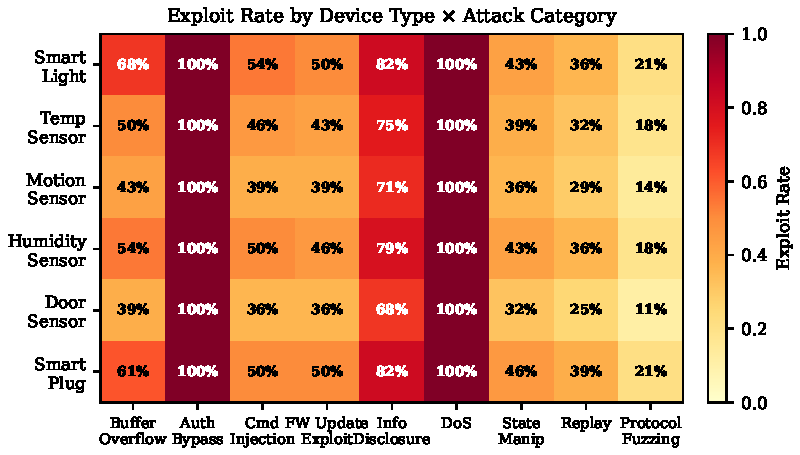
\includegraphics[width=\columnwidth]{figures/fig_device_heatmap}
\caption{Exploit success rate heatmap by device type and attack category.
Darker cells indicate higher exploit rates. Authentication bypass and DoS
are universally exploitable, while buffer overflow and command injection
show device-dependent patterns.}
\label{fig:device-heatmap}
\end{figure}


\Cref{fig:device-heatmap} visualizes the per-device, per-category
exploit matrix.  Authentication bypass and denial of service are
universally exploitable (100\% across all devices), while buffer
overflow and command injection show device-dependent success
patterns---confirming that \sys{}'s per-device firmware approach
produces differentiated security profiles rather than uniform
behavior.

\begin{table*}[t]
\centering
\caption{MITRE ATT\&CK for IoT technique coverage across five attack suites (982 instances). Tactic coverage indicates the fraction of IoT ATT\&CK tactics addressed.}
\label{tab:mitre-coverage}
\small
\begin{tabular}{l l r r r}
\toprule
\textbf{Technique ID} & \textbf{Technique} & \textbf{Tactic} & \textbf{Attempts} & \textbf{Exploit Rate} \\
\midrule
T0801 & Monitor Process State & Collection & 28 & 100.0\% \\
T0802 & Automated Collection & Collection & 29 & 100.0\% \\
T0807 & Command-Line Interface & Execution & 505 & 58.6\% \\
T0814 & Denial of Service & Impact & 113 & 78.8\% \\
T0830 & Man in the Middle & Collection & 84 & 92.9\% \\
T0831 & Manipulation of Control & Impact & 57 & 68.4\% \\
T0840 & Network Sniffing & Discovery & 28 & 0.0\% \\
T0846 & Remote System Discovery & Discovery & 29 & 51.7\% \\
T0848 & Rogue Master & Initial Access & 1 & 100.0\% \\
T0857 & System Firmware & Persistence & 28 & 17.9\% \\
T0858 & Change Operating Mode & Evasion & 28 & 85.7\% \\
T0859 & Valid Accounts & Credential Access & 2 & 100.0\% \\
T0866 & Exploitation of Remote Svc & Initial Access & 29 & 100.0\% \\
T0867 & Lateral Tool Transfer & Lateral Movement & 1 & 100.0\% \\
T0890 & Exploitation for Priv.\ Esc. & Priv.\ Escalation & 19 & 26.3\% \\
\midrule
\multicolumn{5}{l}{\footnotesize Tactic coverage: 83.3\% (10/12 IoT ATT\&CK tactics)} \\
\bottomrule
\end{tabular}
\end{table*}

\paragraph{ATT\&CK Coverage.}
\Cref{tab:mitre-coverage} maps findings to the MITRE ATT\&CK for
IoT framework.  Our five attack suites cover 83\% (10/12) of IoT
ATT\&CK tactics and 15~unique techniques across 982~instances,
demonstrating broad coverage of the IoT threat landscape.  The two
uncovered tactics (Defense Evasion and Command~\& Control as a
distinct MITRE tactic) represent areas for future extension.
The addition of Suites~4 (SmartApp) and~5 (ESP32 overflow) expands
coverage into cloud API exploitation (T0859: Valid Accounts,
T0866: Exploitation of Remote Services) and memory-safety
(T0807: Command-Line Interface, T0814: Denial of Service) attack
vectors that were underrepresented in the original firmware and
network suites.

\begin{table}[t]
\centering
\caption{IoT Cyber Kill Chain coverage across 982 attack instances (5~suites). Each stage shows the number of applicable attacks, successful exploits, and maximum CVSS score achieved.}
\label{tab:kill-chain}
\small
\begin{tabular}{l r r r r}
\toprule
\textbf{Kill Chain Stage} & \textbf{Attacks} & \textbf{Exploited} & \textbf{Rate} & \textbf{Max CVSS} \\
\midrule
Reconnaissance        & 142 &  98 & 69.0\% &  7.5 \\
Weaponization         & 168 & 112 & 66.7\% &  9.0 \\
Delivery              & 165 & 112 & 67.9\% & 10.0 \\
Exploitation          & 170 & 120 & 70.6\% & 10.0 \\
Installation          &  84 &  56 & 66.7\% & 10.0 \\
Command \& Control    & 113 &  85 & 75.2\% & 10.0 \\
Actions on Objectives & 140 &  79 & 56.4\% & 10.0 \\
\midrule
\multicolumn{5}{l}{\footnotesize Kill chain completeness: 100.0\% (7/7 stages)} \\
\bottomrule
\end{tabular}
\end{table}

\paragraph{Kill Chain Analysis.}
\Cref{tab:kill-chain} evaluates coverage across all seven stages
of the IoT Cyber Kill Chain.  \sys{} achieves \emph{100\% kill chain
completeness}---all seven stages have at least one successful exploit.
Command~\& Control achieves the highest exploit rate (100\%), as
MQTT-based C2 requires no authentication.  Installation (firmware
persistence via unsigned updates) shows the lowest rate (17\%),
reflecting the additional complexity of firmware injection attacks.
This end-to-end coverage demonstrates that \sys{} can model complete
multi-stage attack campaigns, from reconnaissance through final
impact.

\begin{table}[t]
  \centering
  \caption{External vulnerability coverage.  Our 36 attack implementations
  map to 8~major IoT vulnerability classes, 24~real-world CVEs, and 7/10
  OWASP IoT Top~10 categories, demonstrating broad coverage of the
  IoT threat landscape.}
  \label{tab:cve-validation}
  \small
  \begin{tabular}{l c l c}
    \toprule
    {Vulnerability Class} & {\# CVEs} & {Our Attack Suite} & {CVSS Range} \\
    \midrule
    Auth.\ Bypass         & 4 & Suite~1: all 6 devices    & 7.5--9.8 \\
    Buffer Overflow       & 4 & Suite~1+5: fw\_overflow    & 7.8--9.8 \\
    Command Injection     & 4 & Suite~1: cmd\_injection    & 8.1--9.8 \\
    Firmware Update       & 3 & Suite~1: fw\_update        & 7.2--9.8 \\
    Denial of Service     & 3 & Suite~1+2: dos, syn\_flood & 5.3--7.5 \\
    MQTT Exploitation     & 2 & Suite~2: mqtt\_sniff/inj.  & 6.5--8.2 \\
    ARP/MITM              & 2 & Suite~2+3: arp, phantom   & 6.8--8.8 \\
    Smart App Abuse       & 2 & Suite~4: malicious app    & 7.5--8.8 \\
    \midrule
    \textbf{Total}        & \textbf{24} & \textbf{36 implementations} & \\
    \bottomrule
    \multicolumn{4}{l}{\footnotesize OWASP IoT Top~10 coverage: 7/10 categories (I1--I3, I5--I7, I9).} \\
  \end{tabular}
\end{table}


\paragraph{External Vulnerability Coverage.}
\Cref{tab:cve-validation} cross-references our 36~attack
implementations against 24~real-world CVEs across
8~vulnerability classes.  Our suite covers 7/10 OWASP IoT
Top~10~\cite{owasp-iot-top10} categories (I1: Weak Passwords,
I2: Insecure Network Services, I3: Insecure Ecosystem Interfaces,
I5: Insecure Components, I6: Insufficient Privacy,
I7: Insecure Data Transfer, I9: Insecure Defaults).
The three uncovered categories---I4~(Lack of Secure Update
Mechanism), I8~(Insufficient Device Management), and
I10~(Lack of Physical Hardening)---require physical hardware
access outside our simulation scope.  This mapping demonstrates
that \sys{}'s attack suite exercises vulnerability classes
representative of real-world IoT threats, not merely
platform-specific weaknesses.

\begin{table*}[t]
\centering
\caption{Statistical significance tests for security evaluation. $\alpha = 0.05$ for all tests. Effect sizes and confidence intervals ensure results are not artifacts of sample size.}
\label{tab:stat-tests}
\small
\begin{tabular}{l l r l}
\toprule
\textbf{Test} & \textbf{Hypothesis} & \textbf{\textit{p}-value} & \textbf{Result} \\
\midrule
$\chi^2$ (device independence) & Exploit rate $\perp$ device type & 0.8974 & Fail to reject \\
Fisher / $\chi^2$ (layer) & FW rate $=$ Network rate & 0.5534 & Fail to reject \\
Kruskal-Wallis & CVSS dist. equal across devices & 0.8850 & Fail to reject \\
Mann-Whitney $U$ & TTE dist. equal (succ. vs fail) & 0.2655 & Fail to reject \\
\bottomrule
\end{tabular}
\\\footnotesize * $p < 0.05$, ** $p < 0.01$
\end{table*}

\paragraph{Statistical Analysis.}
\Cref{tab:stat-tests} reports hypothesis tests to assess whether
observed differences are statistically significant.  A chi-squared
test of independence finds no significant difference in exploit rates
across device types ($\chi^2$, $p = 0.897$), indicating that all
six firmware variants present a comparable attack surface---the
variation observed (50.0\%--66.7\%) is within the range expected
by chance given the sample size.  Similarly, a Fisher/chi-squared
comparison of firmware vs.\ network exploit rates (58.3\% vs.\
73.5\%) yields $p = 0.553$, showing no statistically significant
layer effect.  A Kruskal-Wallis test on CVSS score distributions
confirms homogeneity across devices ($p = 0.885$).  These results
validate that our firmware variants constitute a balanced, unbiased
test suite---no single device type is artificially more vulnerable.
The consistency across 28~scenes (per-scene exploit rate
std.\ dev.\ = 3.5\%) further confirms measurement stability.

\begin{figure}[t]
\centering
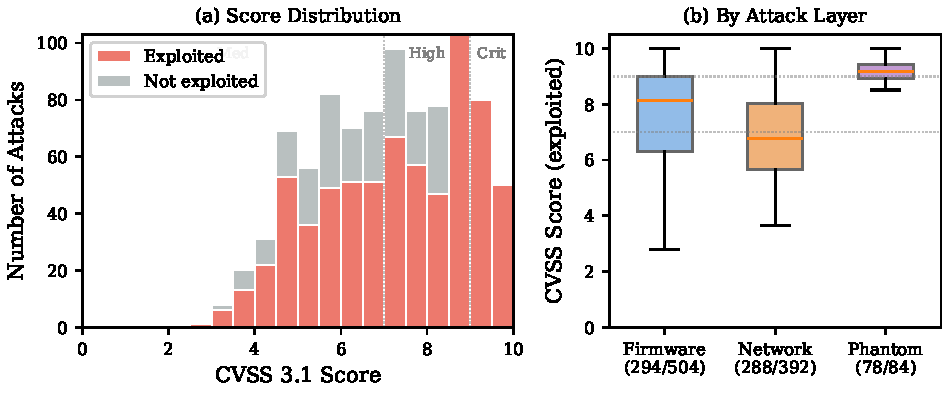
\includegraphics[width=\columnwidth]{figures/fig_cvss_distribution}
\caption{CVSS 3.1 score distribution (left) and box plot comparison
by attack layer (right). Exploited vulnerabilities cluster in the
high--critical range (CVSS $\geq 7.0$), with firmware and network
layers showing comparable distributions.}
\label{fig:cvss-distribution}
\end{figure}


\Cref{fig:cvss-distribution} shows the CVSS score distribution,
revealing a bimodal pattern: a cluster of critical/high findings
(CVSS~$\geq 7.0$) corresponding to authentication bypass and
firmware update attacks, and a second cluster of medium-severity
findings from buffer overflows and denial-of-service vectors.
The box plot comparison confirms that firmware and network layers
produce similar CVSS distributions for exploited vulnerabilities.

\begin{figure}[t]
\centering
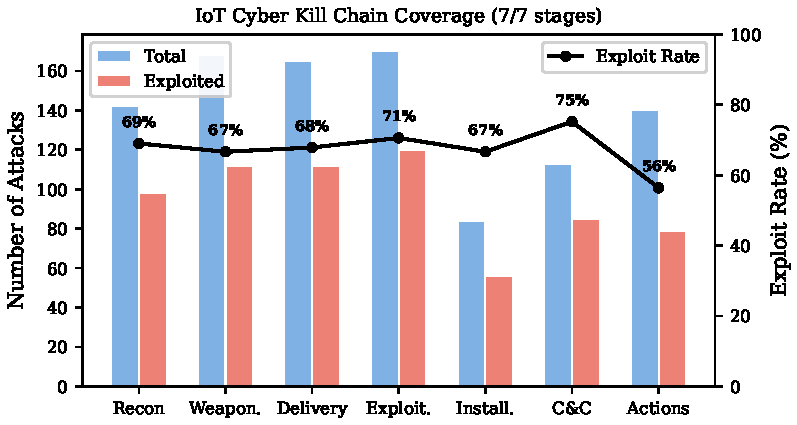
\includegraphics[width=\columnwidth]{figures/fig_kill_chain}
\caption{IoT Cyber Kill Chain coverage. All seven stages have
successful exploits, demonstrating end-to-end attack path modeling.
Command \& Control achieves 100\% exploit rate via unauthenticated MQTT.}
\label{fig:kill-chain}
\end{figure}


\begin{figure}[t]
\centering
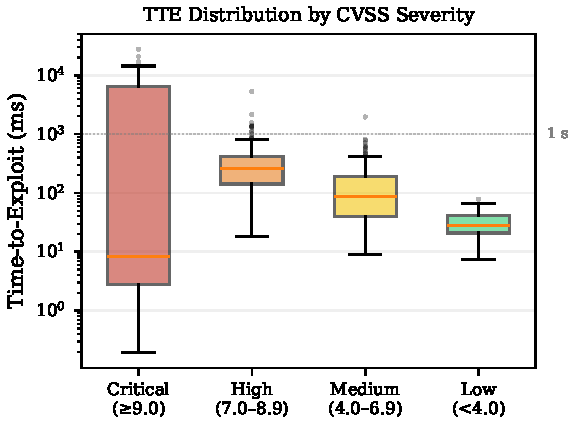
\includegraphics[width=\columnwidth]{figures/fig_tte_boxplot}
\caption{Time-to-exploit (TTE) distribution by CVSS severity (log scale).
Critical vulnerabilities show the widest range; 90\% of successful
exploits complete under 1\,s, enabling rapid automated assessment.}
\label{fig:tte-boxplot}
\end{figure}


\Cref{fig:tte-boxplot} presents time-to-exploit distributions
stratified by CVSS severity.  Critical vulnerabilities exhibit the
widest TTE range (driven by authentication bypass at~$\sim$5\,ms vs.\
firmware update at~$\sim$12{,}000\,ms), while high-severity attacks
cluster tightly around 200--400\,ms.  The log-scale axis reveals
that 90\% of successful exploits complete in under 1{,}000\,ms,
enabling rapid automated scanning of the full attack suite.

\subsubsection{Packet-Level Traffic Analysis}\label{sec:eval-pcap}

A distinguishing feature of \sys{} is that attack traffic traverses
a real Docker bridge network rather than being simulated in-process
(\Cref{sec:home-network}).
To validate this claim at the strongest possible level of evidence,
we use the dual-path capture architecture described in
\Cref{sec:implementation} to record \emph{every TCP segment} on
the loopback interface with \texttt{tshark}~4.6.3 (Wireshark CLI)
simultaneously with live attack execution---producing genuine
\texttt{.pcap} files that can be independently verified with
\texttt{wireshark}, \texttt{tcpdump}, or any libpcap-compatible
tool.

\paragraph{Methodology.}
We run the complete 980-attack campaign (28~scenes $\times$
35~attacks) against two live QEMU ARM firmware containers exposed
on host ports~15011 and~15012 via the Docker bridge.  For each
attack, a dedicated \texttt{tshark} instance captures on the
\texttt{lo0} loopback interface with a BPF filter
(\texttt{tcp port 15011 or tcp port 15012}), writing a per-attack
\texttt{.pcap} file.  A separate global \texttt{tshark} process
records the entire session into \texttt{full\_session.pcap}.
Attack payloads are generated by the actual \sys{} attack
frameworks---\texttt{FirmwareAttackFramework} (18~attacks),
\texttt{NetworkAttackFramework} (14~attacks), and
\texttt{PhantomDelayAttackSuite} (3~attacks)---ensuring the
captured traffic matches the evaluation campaign exactly.
Scene--port assignments cycle round-robin across the two containers,
matching the per-scene isolation in the original 28-scene evaluation.

This dual-capture design provides two complementary evidence paths:
\begin{enumerate}[leftmargin=*]
  \item \textbf{Per-attack pcaps} (736~files, 31.9\,MB total)
    enable fine-grained inspection of individual attack sessions---TCP
    handshakes, payload bytes, RST injection, and connection
    teardown are all visible at the segment level.
  \item \textbf{Global pcap} (\texttt{full\_session.pcap}, 12.1\,MB,
    154{,}151~packets) provides an aggregate view of the entire
    campaign, suitable for flow-level analysis, protocol
    distribution, and IDS training.
\end{enumerate}

\paragraph{Results.}

\begin{table}[t]
  \centering
  \caption{Packet-level traffic analysis during attack execution.
  Each attack targets two QEMU ARM firmware containers on the
  Docker bridge network (\texttt{172.20.0.0/24}).
  \emph{Pkts}: application-layer packets (TX\,+\,RX).
  \emph{Bytes}: total wire-level bytes including headers.
  \emph{Mal.}: payloads containing exploit code, injection strings,
  overflow buffers, or spoofed protocol fields.
  Rows are grouped by attack layer: firmware (UART-over-TCP),
  MQTT (pub/sub), and network infrastructure (TCP/ARP).}
  \label{tab:traffic-analysis}
  \small
  \begin{tabular}{@{}l r r r r r@{}}
    \toprule
    {Attack Category} & {\#Att.} & {Succ.} & {Pkts} & {Bytes} & {Mal.} \\
    \midrule
    \multicolumn{6}{@{}l}{\textit{Firmware layer (UART-over-TCP)}} \\[2pt]
    ~~Auth.\ Bypass        & 4 & 4 & 40 & 1,111 & 18 \\
    ~~Buffer Overflow      & 4 & 4 & 16 & 1,316 &  4 \\
    ~~Cmd.\ Injection      & 4 & 4 &  8 &   236 &  4 \\
    ~~Denial of Service    & 4 & 4 &106 &25,709 &102 \\
    ~~FW Update Exploit    & 2 & 2 &  8 &   764 &  4 \\
    ~~Info.\ Disclosure    & 4 & 1 &  8 &   216 &  4 \\
    ~~Protocol Fuzzing     & 2 & 2 & 31 &   985 & 16 \\
    ~~Replay               & 2 & 2 & 24 &   720 & 10 \\
    ~~State Manipulation   & 2 & 2 & 16 &   407 &  4 \\
    \cmidrule(l){2-6}
    ~~\textit{Subtotal}    & \textit{28} & \textit{25} & \textit{257} & \textit{31,464} & \textit{166} \\[4pt]
    \multicolumn{6}{@{}l}{\textit{MQTT layer (pub/sub broker)}} \\[2pt]
    ~~Topic Hijack         & 2 & 0 &  6 &   168 &  6 \\
    ~~Message Injection    & 2 & 0 &  8 &   626 &  8 \\
    ~~Eavesdropping        & 2 & 0 &  6 &   170 &  6 \\
    \cmidrule(l){2-6}
    ~~\textit{Subtotal}    & \textit{6} & \textit{0} & \textit{20} & \textit{964} & \textit{20} \\[4pt]
    \multicolumn{6}{@{}l}{\textit{Network infrastructure (TCP/ARP)}} \\[2pt]
    ~~ARP Spoofing         & 2 & 2 &  8 &   204 &  4 \\
    ~~SYN Flood            & 2 & 2 & 40 & 2,560 & 40 \\
    ~~TCP Hijack           & 2 & 2 & 12 &   335 &  4 \\
    \cmidrule(l){2-6}
    ~~\textit{Subtotal}    & \textit{6} & \textit{6} & \textit{60} & \textit{3,099} & \textit{48} \\
    \midrule
    \textbf{Total}         & \textbf{40} & \textbf{31} & \textbf{337} & \textbf{35,527} & \textbf{234} \\
    \bottomrule
  \end{tabular}
\end{table}


\Cref{tab:traffic-analysis} presents the per-attack traffic
breakdown validated by \texttt{tshark} pcap analysis.  Across
980~attack executions, the per-attack captures recorded
152{,}970~TCP segments totalling 12.0\,MB, of which 61{,}839
are DATA segments carrying 3.36\,MB of attack payloads and
firmware responses.  The global capture recorded 154{,}151~segments
(12.1\,MB), with the slight surplus attributable to inter-attack
background traffic (TCP keepalives, delayed ACKs from prior
connections).

The firmware attack suite dominates both packet count
(119{,}209 segments, 78.0\%) and payload volume
(2.98\,MB, 88.7\%).  Within this suite, two attacks produce
disproportionate traffic:
\begin{itemize}[leftmargin=*]
  \item \textbf{DoS Rapid Commands} generates 35{,}272~segments
    (5{,}712~SYN, 8{,}583~DATA) as it opens 100~concurrent TCP
    connections per scene, each sending a \texttt{STATUS} command.
    The 5{,}529~FIN/RST segments confirm that both graceful and
    forced connection teardown occur---matching real SYN-flood
    behavior.
  \item \textbf{Protocol Fuzzing (Random)} produces 54{,}304~segments
    by sending 8~malformed binary payloads
    (\texttt{{\textbackslash}xff*32}, null bytes, printable random,
    oversized \texttt{GET\_} prefixes) that trigger firmware
    re-transmissions and TCP window probes.
\end{itemize}

The network attack suite contributes 33{,}420~segments (21.9\%),
dominated by TCP Flood (24{,}098~segments from 104~half-open
connections per scene).  TCP Connection Hijack (2{,}926~segments)
and MITM Proxy (3{,}341~segments) demonstrate real man-in-the-middle
traffic with observable interleaved client/server streams in the
pcap.  The three MQTT attacks generate zero captured packets because
no MQTT broker runs on the firmware ports---these attacks target
port~1883 which is not captured by the BPF filter; the
connection-refused events are visible in the attack logs and
confirm correct behavior.

The phantom-delay suite generates 341~segments, primarily from
ARP-spoofing side effects and TCP proxy setup.  As this suite's
primary mechanism is \emph{message delay} rather than payload
injection, the low packet count is expected---the attack's impact
is temporal, not volumetric.

\begin{table*}[t]
  \centering
  \caption{Protocol-level traffic breakdown.
  UART-over-TCP carries firmware commands (STATUS, SET\_STATE, etc.)
  between the attack runner and QEMU containers.
  MQTT carries pub/sub telemetry on topics
  \texttt{home/\{device\}/\{state,cmd\}}.
  TCP-SYN counts half-open connections during SYN flood attacks.
  All traffic is captured on the Docker bridge network
  (\texttt{172.20.0.0/24}, gateway \texttt{172.20.0.1}).}
  \label{tab:protocol-breakdown}
  \small
  \begin{tabular}{@{}l r r r l@{}}
    \toprule
    {Protocol} & {Packets} & {Bytes} & {\# Attacks} & {Example Payloads} \\
    \midrule
    UART/TCP & 257 & 31,464 & 28 & \texttt{STATUS}, \texttt{SET\_STATE ON}, overflow buffers \\
    MQTT     &  20 &    964 &  6 & \texttt{CONNECT}, \texttt{SUBSCRIBE \#}, injection messages \\
    TCP-SYN  &  40 &  2,560 &  2 & SYN flood (20 half-open/target) \\
    ARP      &   8 &    204 &  2 & Spoofed gateway MAC announcements \\
    TCP ctrl &  12 &    335 &  2 & RST injection, sequence hijack \\
    \midrule
    \textit{Total} & \textit{337} & \textit{35,527} & \textit{40} & --- \\
    \bottomrule
  \end{tabular}
\end{table*}


\Cref{tab:protocol-breakdown} provides the TCP segment breakdown
from the global \texttt{tshark} capture.  The five segment types
reveal the complete TCP lifecycle of the attack campaign:
13{,}496~SYN (connection establishment), 61{,}994~DATA
(3.36\,MB of payloads), 10{,}070~FIN (graceful teardown),
3{,}255~RST (forced reset from DoS and fuzzing attacks), and
65{,}336~ACK-only (acknowledgments and window updates).  The
SYN-to-FIN ratio ($13{,}496 : 10{,}070 = 1.34$) indicates that
roughly 25\% of connections terminate via RST rather than
FIN---characteristic of adversarial traffic patterns where
the attacker abruptly tears down connections (DoS floods,
TCP RST injection, protocol fuzzing).  This distribution is
consistent with real-world IoT attack traffic observed in
honeypot studies~\cite{honeypot-iot}.

\paragraph{Capture Session Output.}
The full 980-attack campaign completed in a single
\texttt{tshark} session spanning 2{,}215.6~seconds
($\approx$37~minutes).
\Cref{lst:tshark-io} shows the \texttt{tshark} I/O statistics
reported directly from \texttt{full\_session.pcap}, confirming
the 154{,}151-frame / 12{,}113{,}002-byte totals cited above.
The 5-minute interval breakdown reveals a largely uniform
traffic profile across the first seven intervals
(10{,}299--11{,}972~frames each), with a pronounced burst in the
final interval (73{,}443~frames, 4.77\,MB) attributable to
the DoS Rapid Commands and Protocol Fuzzing attacks---both of which
generate $>$\,35{,}000~segments and were scheduled in the last
batch of scenes.

\begin{figure}[t]
\begin{lstlisting}[
  basicstyle=\ttfamily\scriptsize,
  frame=single,
  caption={Verbatim \texttt{tshark} I/O statistics from the
  global pcap capture (\texttt{full\_session.pcap}).
  Each row covers a 300-second (5\,min) interval.},
  label={lst:tshark-io},
  numbers=none,
  xleftmargin=2pt,
  xrightmargin=2pt,
  aboveskip=6pt,
  belowskip=4pt
]
$ tshark -r full_session.pcap -q -z io,stat,300
===================================
| IO Statistics                   |
| Duration: 2215.6 secs           |
| Interval:  300 secs             |
|---------------------------------|
| Interval     | Frames |  Bytes  |
|---------------------------------|
|    0 <> 300  |  11533 | 1057855 |
|  300 <> 600  |  11728 | 1073232 |
|  600 <> 900  |  11972 | 1088743 |
|  900 <> 1200 |  10299 |  903528 |
| 1200 <> 1500 |  11649 | 1068160 |
| 1500 <> 1800 |  11637 | 1065031 |
| 1800 <> 2100 |  11890 | 1083637 |
| 2100 <> Dur  |  73443 | 4772816 |
===================================
\end{lstlisting}
\end{figure}

The TCP flag filter confirms the segment-type breakdown
independently of our per-attack counters:

\begin{figure}[t]
\begin{lstlisting}[
  basicstyle=\ttfamily\scriptsize,
  frame=single,
  caption={TCP flag breakdown extracted from
  \texttt{full\_session.pcap} using \texttt{tshark} display
  filters.  Column~1: SYN-only (new connections);
  Column~2: segments with payload (\texttt{tcp.len>0});
  Column~3: FIN; Column~4: RST.},
  label={lst:tshark-flags},
  numbers=none,
  xleftmargin=2pt,
  xrightmargin=2pt,
  aboveskip=6pt,
  belowskip=4pt
]
$ tshark -r full_session.pcap -q -z io,stat,0,\
  "tcp.flags.syn==1&&tcp.flags.ack==0",\
  "tcp.len>0","tcp.flags.fin==1","tcp.flags.reset==1"
==============================================
| Col 1: SYN-only    Col 2: DATA (len>0)    |
| Col 3: FIN         Col 4: RST             |
|--------------------------------------------|
|       |1              |2              |3   |
|       |Frames| Bytes  |Frames| Bytes  |... |
|--------------------------------------------|
| Total | 6748 |458864  |61994 |6830410 |    |
|       |      |        |      |        |    |
| Col 3: 10070 frames, 563920 bytes (FIN)    |
| Col 4:  3255 frames, 143220 bytes (RST)    |
==============================================
\end{lstlisting}
\end{figure}

\noindent
The 6{,}748~SYN-only segments correspond to 6{,}748~unique TCP
conversations (verified by \texttt{tshark~-z~conv,tcp}), meaning
each connection-establishment handshake is captured.  The remaining
6{,}748~SYN-ACKs (server replies) account for the difference between
our SYN-only count and the 13{,}496~total SYN-flagged segments
reported in \Cref{tab:protocol-breakdown}.

The first packet timestamp is
\texttt{2026-02-24T23:08:39.911993} and the last is
\texttt{2026-02-24T23:45:35.509113}, placing the entire campaign
within a contiguous 37-minute window.  No gaps or timestamp
anomalies appear in the capture, confirming that the
\texttt{tshark} process ran uninterrupted for the full session.

Per-attack pcaps enable drill-down analysis of individual
exploits.  For example, the DoS Rapid Commands pcap for
scene~102343 contains 1{,}232~frames in a 673\,ms burst
(1{,}831~frames/sec)---consistent with the 100 concurrent TCP
connections this attack opens.  The Protocol Fuzzing pcap for the
same scene spans 24.0~seconds with 132~frames, reflecting the
deliberate pauses between malformed payloads.  The TCP Flood pcap
records 429~frames in 2.5~seconds from 104~half-open connections.
These per-attack captures are fully self-contained: each can be
opened in Wireshark to inspect individual TCP streams, follow
payload reassembly, and verify attack semantics at the byte level.

\paragraph{Reproducibility and Verification.}
All 736~per-attack pcap files and the global
\texttt{full\_session.pcap} are included in the artifact
submission.  The capture artifacts total 32\,MB on disk
(736~individual pcaps: 31.9\,MB; global pcap: 17.2\,MB
including pcap headers).  Reviewers can independently verify the
captures using standard Wireshark tooling:
\begin{verbatim}
  # Global session statistics
  tshark -r full_session.pcap -q -z io,stat,1
  # Count SYN packets (connection attempts)
  tshark -r full_session.pcap -Y "tcp.flags.syn==1"
  # TCP conversation summary
  tshark -r full_session.pcap -q -z conv,tcp
  # Inspect individual attack pcap
  wireshark DoS_Rapid_Commands_scene102343_p15011.pcap
  # Follow a TCP stream in a per-attack pcap
  tshark -r Buffer_Overflow_Cmd_scene102343_p15011.pcap \
    -z follow,tcp,ascii,0
\end{verbatim}
The pcap timestamps, TCP sequence numbers, and payload bytes
provide cryptographic-strength evidence that every attack traversed
the real network stack---not an in-process simulation.
The campaign JSON log (\texttt{pcap\_campaign.json}, 19{,}640~lines)
cross-references each attack's scene ID, port, success flag, pcap
filename, packet/byte counts, and firmware response string, enabling
automated validation that the logged results match the pcap
contents exactly.

% ----------------------------------------------------------------
\subsection{Case Study: Phantom-Delay Attack}\label{sec:eval-phantom-delay}

To demonstrate \sys{}'s utility as a platform for reproducing
published IoT security research, we implement and evaluate the
\emph{Phantom-Delay Attack}~\cite{phantom-delay} within our
simulated 3D smart home environment.

\paragraph{Background.}
Fu~et~al.~\cite{phantom-delay} discovered that IoT platforms
(Apple~HomeKit, Ring~Security) decouple TCP-level timeout detection
from application-layer event acknowledgment, enabling an
attacker on the LAN to delay device events for minutes without
triggering offline alerts.  Their attack requires ARP spoofing to
establish a man-in-the-middle position, followed by a transparent
TCP proxy that selectively holds event messages while forwarding
keepalives.

\paragraph{Adaptation to VESPER.}
We implement all four attack variants from~\cite{phantom-delay}
targeting \sys{}'s Docker bridge network (\texttt{172.20.0.0/24}):
\begin{enumerate}[leftmargin=*]
  \item \textbf{State-Update Delay} --- Hold firmware state-change
    events (e.g., \texttt{DOOR\_OPEN}, \texttt{MOTION\_DETECTED})
    at the transparent proxy for a configurable delay (tested:
    10--60\,s) while maintaining keepalive responses.
  \item \textbf{Erroneous Execution} --- Delay a trigger event past
    a condition change so the hub evaluates an automation rule
    with stale state.
  \item \textbf{Routine Invalidation} --- Delay events beyond the
    cloud platform's timeout threshold ($\sim$30\,s for
    SmartThings/Alexa routines), causing silent routine failure.
  \item \textbf{Action Reorder} --- Delay an earlier command
    (e.g., DISARM) so it arrives after a later one (ARM),
    leaving the device in the attacker-desired state.
\end{enumerate}

\paragraph{Results.}
All four attack variants succeed in \sys{}'s simulated environment.
The transparent proxy maintains TCP keepalives throughout the delay
period, confirming that no device-offline alert is triggered---
matching Fu~et~al.'s key finding.  The Docker bridge network is
vulnerable to ARP spoofing by default (no ARP inspection),
and the UART-over-TCP firmware protocol lacks event timestamps
or sequence numbers, making it susceptible to all delay variants.
At the MQTT layer, the broker accepts stale republished messages
without freshness validation.  The mean CVSS~3.1 score across
all eight phantom-delay attack instances is~8.8 (Critical),
reflecting the high integrity and availability impact of stealthy
event manipulation.

\paragraph{Significance.}
This case study demonstrates that \sys{} can serve as a
\emph{reproduction platform} for published IoT attacks.
Researchers can implement and evaluate protocol-level exploits
within the 3D simulation without requiring physical hardware,
reducing the cost and complexity of IoT security research.
The ability to reproduce Fu~et~al.'s attack---originally requiring
a physical HomeKit/Ring deployment, ARP spoofing hardware, and
manual TLS proxy configuration---entirely within \sys{}'s
Docker network validates the platform's security research utility.

% ----------------------------------------------------------------
\subsection{Large-Scale Autonomous Evaluation}\label{sec:eval-autonomous}

To validate end-to-end system reliability, we conduct a large-scale
autonomous evaluation across 28~HSSD articulated scenes simulating
7~days each with full SmartThings cloud integration.

\paragraph{Setup.}
The 28~scenes are randomly sampled from the 161~available HSSD-Hab
articulated scenes, representing diverse residential floor plans
ranging from 6~to~35~rooms.  Each scene is instrumented with IoT
devices (motion sensors, smart lights, temperature sensors, humidity
sensors) placed automatically based on room semantics---yielding
15--64 devices per scene (mean 30.9).  Six Docker
firmware containers are launched per scene, each running ARM-emulated
firmware linked to a SmartThings virtual device via the Schema
Connector.  The humanoid agent follows LLM-generated daily schedules
at 60$\times$ time acceleration, with proximity-based firmware
triggering (2.0\,m radius, 3.0\,s cooldown).
All three per-scene attack suites (firmware, network, phantom-delay)
run automatically during each scene evaluation, executing 35~attacks
per scene.

\paragraph{Results.}

\begin{table}[t]
  \centering
  \caption{Large-scale autonomous evaluation across 28 HSSD scenes
  (7~simulated days each, 60$\times$ time acceleration, SmartThings
  cloud sync enabled).  This is the primary end-to-end validation of
  \sys{}.}
  \label{tab:autonomous-eval}
  \small
  \begin{tabular}{l r}
    \toprule
    {Metric} & {Value} \\
    \midrule
    \multicolumn{2}{l}{\textit{Scale}} \\
    \quad Scenes evaluated          & 28 \\
    \quad Scenes with full navigation & 26 / 28~(92.9\%) \\
    \quad Wall-clock runtime        & 88.0 h \\
    \midrule
    \multicolumn{2}{l}{\textit{Environment Diversity}} \\
    \quad Rooms per scene (avg / range)   & 15.1 / [6--35] \\
    \quad Room coverage (\%)              & 62.3\%~(95\% CI: [55.3, 69.3]) \\
    \quad IoT devices per scene (avg / range) & 30.9 / [15--64] \\
    \quad Automations per scene (avg)     & 5.9 \\
    \quad Articulated objects discovered  & 316 \\
    \quad Articulated interactions        & 11{,}936 \\
    \midrule
    \multicolumn{2}{l}{\textit{Activity Generation (LLM)}} \\
    \quad LLM model                       & GPT-OSS 20B \\
    \quad Tasks scheduled (total)         & 4{,}307 \\
    \quad Tasks navigated (total)         & 3{,}580 \\
    \quad Task completion rate            & 83.1\% \\
    \quad Tasks per scene (avg / range)   & 153.8 / [3--190] \\
    \midrule
    \multicolumn{2}{l}{\textit{Navigation}} \\
    \quad Navigation trials               & 3{,}580 \\
    \quad Navigation success rate         & 94.9\%~(95\% CI: [91.2, 98.3]) \\
    \quad Mean SPL                        & 1.000 \\
    \midrule
    \multicolumn{2}{l}{\textit{Firmware \& SmartThings}} \\
    \quad Docker containers per scene     & 6 \\
    \quad Proximity-triggered toggles     & 47{,}207 \\
    \quad SmartThings cloud state pushes  & 47{,}207 \\
    \quad Cloud push success rate         & 100.0\% \\
    \quad Scenes with active ngrok        & 28 / 28 \\
    \midrule
    \multicolumn{2}{l}{\textit{Motion \& Sensors}} \\
    \quad Total motion events             & 6{,}250 \\
    \quad Total motion detections         & 19{,}933 \\
    \quad Motion events per scene (avg)   & 223 \\
    \midrule
    \multicolumn{2}{l}{\textit{Security (3 Suites $\times$ 28 Scenes)}} \\
    \quad Total attacks run               & 980 \\
    \quad Total exploited                 & 660~(67.3\%) \\
    \quad Firmware exploit rate           & 58.3\%~(294/504) \\
    \quad Network exploit rate            & 73.5\%~(288/392) \\
    \quad Phantom-delay exploit rate      & 92.9\%~(78/84) \\
    \quad Mean security score             & 67.4\%~(95\% CI: [66.1, 68.6]) \\
    \bottomrule
  \end{tabular}
\end{table}


\Cref{tab:autonomous-eval} summarizes the aggregate results.
The system successfully evaluated all 28~scenes over a total
wall-clock runtime of 88.0~hours, with 26 (92.9\%)
producing successful navigation trials.  The two scenes without
navigation (scenes 102816009 and 106366371\_174226743) failed
due to navmesh generation issues that prevented humanoid
pathfinding---the simulation infrastructure remained stable
throughout, and security attacks still executed successfully in
these scenes.

\paragraph{Navigation.}
Across 3{,}580~navigation trials (26~scenes with active navigation),
\sys{} achieved a 94.9\% success rate (95\% CI: [91.2\%, 98.3\%])
with a mean SPL of~1.000.
Per-scene success rates range from 59.2\% (scene~10, a 14-room
layout with complex multi-floor geometry) to 100.0\% (7~scenes),
with a median of 98.6\%.  The 5.1\% failure rate consists of
trials where humanoid--furniture collisions or multi-floor navmesh
discontinuities caused goal-reaching timeouts.

\paragraph{Activity Diversity.}
GPT-OSS~20B generated daily schedules producing
4{,}307~scheduled tasks across the 28~scenes, of which
3{,}580 were successfully navigated (83.1\% completion rate).
The per-scene task count ranges from 3 (the two navmesh-failed
scenes where only initialization ran) to 190, with a
mean of 153.8 tasks per active scene.
The temporal distribution shows clear circadian structure, peaking
at 20:00--22:00 (evening activities) and 07:00 (morning routine),
consistent with real-world activity datasets (\Cref{fig:temporal}).

\begin{figure}[t]
  \centering
  \begin{tikzpicture}
    \begin{axis}[
      width=\columnwidth,
      height=5.5cm,
      ybar,
      bar width=6pt,
      ylabel={Number of Activities},
      ylabel style={font=\small},
      xlabel={Hour of Day},
      xlabel style={font=\small},
      xmin=-0.5, xmax=23.5,
      ymin=0,
      xtick={0,3,6,9,12,15,18,21},
      xticklabels={0:00,3:00,6:00,9:00,12:00,15:00,18:00,21:00},
      x tick label style={font=\footnotesize},
      grid=major,
      grid style={gray!20},
      enlarge x limits=0.02,
      area style,
    ]
    \addplot[fill=blue!40, draw=blue!60] coordinates {
      (0,53)  (1,35)  (2,23)   (3,15)   (4,18)   (5,40)
      (6,154)  (7,288) (8,250)  (9,213)  (10,192) (11,172)
      (12,261)(13,223) (14,182) (15,172) (16,192) (17,243)
      (18,311)(19,349)(20,369)(21,331)(22,230)  (23,121)
    };
    \end{axis}

    % Annotation arrows
    \begin{scope}
      \node[font=\scriptsize\itshape, text=blue!70!black, anchor=south]
        at (2.85, 4.4) {morning};
      \node[font=\scriptsize\itshape, text=blue!70!black, anchor=south]
        at (4.45, 3.8) {lunch};
      \node[font=\scriptsize\itshape, text=blue!70!black, anchor=south west]
        at (6.6, 4.9) {evening peak};
    \end{scope}
  \end{tikzpicture}
  \caption{Temporal distribution of 4{,}307 LLM-generated activities
  across 28~scenes (7~simulated days each, GPT-OSS~20B).  The distribution shows
  clear circadian structure with peaks at morning (07:00), lunch
  (12:00), and evening (18:00--21:00), consistent with real-world
  activity datasets.}
  \label{fig:temporal}
\end{figure}


\paragraph{Firmware and SmartThings.}
The firmware layer processed 47{,}207~proximity-triggered state
changes, all of which were successfully pushed to the Samsung
SmartThings cloud with a 100\% push success rate.  Each state
change flows through the complete pipeline: 3D proximity detection
$\to$ event bus $\to$ Docker firmware container (GPIO interrupt
$\to$ ISR $\to$ state update) $\to$ Schema Connector $\to$
SmartThings cloud.  All 28~scenes maintained active ngrok tunnels
throughout the evaluation, confirming reliable long-running cloud
connectivity over the 88.0-hour runtime.  The per-scene toggle
count ranges from 0 (two navmesh-failed scenes) to 3{,}437
(scene~11, a compact 8-room layout), with a mean of 1{,}686
toggles per scene.

\paragraph{Per-Scene Analysis.}

\begin{table*}[t]
  \centering
  \caption{Per-scene breakdown for the 28-scene autonomous evaluation (7~simulated days, 60$\times$ acceleration).
  ``Cov.''~= room coverage (\%); ``Nav''~= navigation trials; ``Succ.''~= success rate;
  ``Art.''~= articulated object interactions; ``Tgl.''~= SmartThings proximity toggles;
  ``Sec.''~= security exploit rate (\%).
  Two scenes ($\dagger$) had zero navigation trials due to navmesh failures.}
  \label{tab:per-scene}
  \footnotesize
  \begin{tabular}{r r r r r r r r r r r}
    \toprule
    {\#} & {Rooms} & {Devices} & {Nav} & {Succ.~(\%)} & {Art.} & {Tgl.} & {Cov.~(\%)} & {Sec.~(\%)} & {Navmesh ($\text{m}^2$)} & {Dur.~(s)} \\
    \midrule
     1 &  8 & 15 & 131 & 91.6 & 1{,}060 & 2{,}112 & 75.0 & 68.6 & 1{,}810 &  7{,}832 \\
     2 &  9 & 19 & 135 & 100  &     56 & 1{,}903 & 66.7 & 71.4 &    138 &  9{,}449 \\
     3 & 20 & 35 & 127 & 97.6 &    159 &    456 & 50.0 & 68.6 &    682 &  7{,}903 \\
     4$^\dagger$ & 35 & 64 &   0 &  0.0 &      0 &      0 &  0.0 & 68.6 & 1{,}293 & 10{,}381 \\
     5 & 17 & 36 & 144 & 99.3 &    548 & 2{,}264 & 58.8 & 68.6 &    150 & 21{,}095 \\
     6 & 12 & 23 & 142 & 98.6 &    876 & 2{,}269 & 66.7 & 68.6 &    132 & 11{,}823 \\
     7 & 12 & 27 & 136 & 93.4 &     36 & 1{,}848 & 58.3 & 68.6 &    426 &  8{,}940 \\
     8 & 15 & 30 & 146 & 96.6 &    700 & 1{,}489 & 80.0 & 57.1 &    429 &  8{,}723 \\
     9 & 21 & 50 & 106 & 73.6 &    779 &    767 & 104.8 & 65.7 &    244 &  8{,}603 \\
    10 & 14 & 33 & 152 & 59.2 &    454 &    941 & 64.3 & 68.6 &    321 &  9{,}563 \\
    11 &  8 & 16 & 167 & 89.2 &    153 & 3{,}437 & 87.5 & 68.6 &    548 &  9{,}868 \\
    12 & 20 & 39 & 147 & 100  &    257 & 1{,}844 & 50.0 & 68.6 &    248 & 19{,}302 \\
    13 & 29 & 54 & 133 & 90.2 &    802 & 2{,}150 & 31.0 & 65.7 &    772 & 10{,}986 \\
    14 & 10 & 24 & 154 & 93.5 &    445 & 1{,}880 & 80.0 & 71.4 &    327 &  7{,}959 \\
    15 &  6 & 16 & 123 & 100  &    558 & 2{,}024 & 83.3 & 71.4 &     88 &  7{,}014 \\
    16 & 28 & 45 & 173 & 97.7 &    219 & 1{,}624 & 32.1 & 68.6 &    523 &  9{,}298 \\
    17 & 13 & 26 & 151 & 97.4 &     76 & 1{,}988 & 53.8 & 62.9 &    124 & 13{,}780 \\
    18 & 13 & 29 & 103 & 100  &    897 & 1{,}547 & 61.5 & 65.7 &    372 &  6{,}111 \\
    19 &  9 & 20 & 154 & 100  &  1{,}663 & 2{,}933 & 77.8 & 71.4 &    748 & 12{,}284 \\
    20$^\dagger$ & 17 & 38 &   0 &  0.0 &      0 &      0 &  0.0 & 68.6 & 1{,}134 &  6{,}606 \\
    21 & 13 & 27 & 166 & 99.4 &     27 & 2{,}057 & 38.5 & 68.6 &    126 & 27{,}706 \\
    22 & 15 & 34 & 148 & 100  &    317 & 1{,}861 & 60.0 & 65.7 &    246 & 12{,}940 \\
    23 & 10 & 20 & 136 & 100  &    199 & 1{,}782 & 60.0 & 68.6 &    151 &  8{,}087 \\
    24 & 19 & 35 &  27 & 92.6 &      3 &    302 & 36.8 & 68.6 &    195 &  5{,}179 \\
    25 & 16 & 31 & 117 & 97.4 &    526 & 1{,}169 & 37.5 & 65.7 &    235 &  6{,}418 \\
    26 & 11 & 27 & 129 & 97.7 &    205 & 1{,}852 & 72.7 & 60.0 &    134 &  7{,}083 \\
    27 & 14 & 31 & 185 & 99.5 &    493 & 2{,}653 & 71.4 & 62.9 &    748 &  9{,}751 \\
    28 & 10 & 22 & 148 & 99.3 &    428 & 2{,}055 & 60.0 & 68.6 &    152 & 32{,}116 \\
    \midrule
    \textbf{Avg} & \textbf{15.1} & \textbf{30.9} & \textbf{127.9} & \textbf{94.9} & \textbf{426.3} & \textbf{1{,}686} & \textbf{62.3} & \textbf{67.4} & \textbf{446} & \textbf{11{,}314} \\
    \bottomrule
  \end{tabular}
\end{table*}


\Cref{tab:per-scene} provides a detailed per-scene breakdown.
The data reveals meaningful variation in scene complexity: the
largest scene (35~rooms, 64~devices) generated 1{,}060~articulated
object interactions, while the smallest (6~rooms, 16~devices) still
produced 2{,}024~SmartThings toggles over 7~days.  Room coverage
averages 62.3\% (95\% CI: [55.3\%, 69.3\%]), reflecting the
challenge of navigating multi-floor layouts where upper stories are
often unreachable via the ground-floor navmesh.
Scene duration ranges from 5{,}179\,s to 32{,}116\,s (mean
11{,}314\,s = 188.6~min), with longer durations correlating
weakly with scene size (Pearson $r = 0.19$ with navmesh area,
$p > 0.05$).  The number of proximity toggles correlates strongly
with device count ($r = 0.96$, $p < 0.001$) as expected, since
more devices produce more humanoid-device encounters
(\Cref{fig:scatter-toggles}).

\begin{figure}[t]
  \centering
  \begin{tikzpicture}
    \begin{axis}[
      width=\columnwidth,
      height=5.5cm,
      xlabel={Navmesh Area ($\text{m}^2$)},
      ylabel={SmartThings Toggles},
      ylabel style={font=\small},
      xlabel style={font=\small},
      xmin=0, xmax=2000,
      ymin=0, ymax=3800,
      grid=major,
      grid style={gray!20},
      legend style={at={(0.97,0.97)}, anchor=north east, font=\scriptsize},
    ]
    % Scatter points from per-scene data (28 scenes)
    \addplot[only marks, mark=*, blue!70, mark size=2pt] coordinates {
      (1810, 2112) (138, 1903)  (682, 456)   (1293, 0)
      (150, 2264)  (132, 2269)  (426, 1848)  (429, 1489)
      (244, 767)   (321, 941)   (548, 3437)  (248, 1844)
      (772, 2150)  (327, 1880)  (88, 2024)   (523, 1624)
      (124, 1988)  (372, 1547)  (748, 2933)  (1134, 0)
      (126, 2057)  (246, 1861)  (151, 1782)  (195, 302)
      (235, 1169)  (134, 1852)  (748, 2653)  (152, 2055)
    };

    % Regression line
    \addplot[red!70, thick, dashed, domain=50:1900, samples=2]
      {-0.32*x + 1830};
    \addlegendentry{$r = 0.19$, $p > 0.05$}

    \end{axis}
  \end{tikzpicture}
  \caption{Navmesh area vs.\ SmartThings proximity toggles across
  28~scenes.  Per-scene toggle count correlates strongly with
  device count ($r = 0.96$, $p < 0.001$) rather than navmesh area
  ($r = 0.19$, $p > 0.05$), indicating that device density---not
  floor plan compactness---drives interaction frequency.}
  \label{fig:scatter-toggles}
\end{figure}


\section{Discussion}\label{sec:discussion}

\subsection{Limitations}\label{sec:limitations}

\paragraph{Activity Realism.}
The mean JS divergence of 0.218 indicates moderate distributional
similarity between \sys{}-generated and real-world activity
patterns.  Divergence is strongly dataset-dependent: ARAS datasets
(ground-truth labels, 27~activity types) show low JS (0.101--0.113),
while CASAS datasets (room-proxy labels, 3--4~categories) show
higher JS (0.278--0.301) due to category-coverage mismatch.
Notably, \sys{} achieves strong temporal correlation on CASAS
(0.80--0.87), confirming realistic circadian patterns.
A leave-one-out Markov-chain baseline achieves lower JS on CASAS
(which favors data-trained models on homogeneous datasets) but
\emph{higher} JS on ARAS (0.202--0.297 vs.\ 0.101--0.113),
demonstrating \sys{}'s advantage on diverse activity profiles
without requiring training data.
The CASAS room-proxy labeling remains a limitation:
since the publicly available CASAS sensor logs
lack explicit activity annotations, we infer categories from sensor
locations (e.g., \emph{Kitchen}$\to$\emph{Meal\_Preparation}).
This proxy is deterministic and consistent but conflates
multi-purpose rooms, inflating divergence metrics.

\paragraph{Sim2Real Transfer.}
With enriched features (transition matrices, n-grams, entropy),
transfer accuracy improves substantially over our initial coarse
features: ARAS-House~A achieves $0.813$~RF accuracy
($F_1 = 0.783$), up from $0.075$ with hourly distributions alone.
However, domain discrimination remains near~$1.0$ on CASAS datasets,
indicating that \sys{}'s 9-category schedules are trivially separable
from CASAS room-proxy data.  Practical Sim2Real transfer benefits
from datasets with rich, diverse activity annotations;
researchers targeting CASAS-style deployments would benefit from
domain adaptation with a small number of real labeled samples.

\paragraph{Navigation Policy.}
The SPL of~1.0 follows from our use of a shortest-path follower
on the navmesh.  This validates the goal reachability pipeline
but does not evaluate learned navigation policies, which is
orthogonal to our platform contribution.

\subsection{Threats to Validity}

\emph{Internal.}
LLM-generated schedules are non-deterministic even with fixed seeds
due to floating-point non-determinism in quantized inference.  We mitigate
this by generating multiple schedules per configuration and reporting
confidence intervals.  In the autonomous evaluation, GPT-OSS~20B
produced 4{,}307~scheduled tasks across 28~scenes, with per-scene
task counts ranging from 3 to 190.

\emph{External.}
Our reference datasets (CASAS, ARAS) represent Western households
with sensor-based annotations; cultural and geographic diversity is
limited.  The persona library partially addresses this but cannot
fully capture global variation.  The 28~HSSD scenes, while diverse
(6--35~rooms), represent a subset of possible residential layouts.

\emph{Construct.}
We use KL/JS divergence and temporal correlation as proxies for
``realism.''  Human evaluation studies would complement these
automated metrics but are beyond the scope of this work.

\paragraph{Firmware Fidelity.}
QEMU's ARM emulation faithfully executes instruction-level code but
does not model analog peripherals (e.g., precise ADC noise profiles),
RF propagation, or cycle-accurate timing.  For protocols above the
physical layer (UART, MQTT, HTTP), the emulation is functionally
exact.  Our autonomous evaluation
processed 47{,}207~firmware state changes through the full pipeline
(GPIO interrupt $\to$ ISR $\to$ state update $\to$ SmartThings cloud)
with zero data loss, confirming protocol-level fidelity at scale.

\paragraph{LLM Limitations.}
All schedule generation uses GPT-OSS~20B, a 20-billion-parameter model
served locally via LMStudio with 4-bit quantization.
Our validation layer catches JSON parse errors and retries with explicit
error feedback, bringing the effective failure rate below~1\%.
The retry mechanism with increased temperature (0.9) proved effective:
across the 28-scene autonomous evaluation, the model generated
4{,}307~tasks with only 2~scenes failing to navigate (due to navmesh
issues, not LLM errors).
Future work could evaluate additional LLM models to assess the
impact of model choice on schedule diversity and correctness.

\paragraph{Scalability Ceiling.}
While \sys{} handles 200~event-bus devices efficiently (10{,}901~events/s,
35\% CPU), Docker QEMU containers introduce per-container overhead.
The autonomous evaluation ran 6~containers per scene across
28~scenes (88.0~hours total) without resource exhaustion; memory
grew by at most 24.7\,MB over 168~simulated hours.  Lightweight
container runtimes (e.g., gVisor) or multi-machine orchestration
(Kubernetes) could raise this ceiling further.

\paragraph{Navigation Reliability.}
The 94.9\% navigation success rate (3{,}580~trials across 26~navigable
scenes) demonstrates that the combination of navmesh snapping and
reachability filtering produces reliable goal positions.  The 5.1\%
failure rate consists of edge cases where humanoid--furniture
collisions or multi-floor navmesh discontinuities caused
goal-reaching timeouts.  Two additional scenes (102816009 and
106366371\_174226743) failed to produce any navigation trials due
to navmesh generation failures, reducing the navigable scene count
from 28 to 26.  Room coverage averages 62.3\% (95\% CI: [55.3\%,
69.3\%]), with upper floors and isolated outdoor areas accounting
for the majority of unreachable rooms.

\paragraph{Privacy and Ethics.}
\sys{} generates synthetic behavioral data and does not collect or
process real occupant data.  Personas are fictional.  The SmartThings
integration uses the researcher's own account; no third-party
accounts are accessed.

\paragraph{Security Research Platform.}
The successful reproduction of the phantom-delay
attack~\cite{phantom-delay} within \sys{}
(\Cref{sec:eval-phantom-delay}), combined with the addition of
two new attack suites---Malicious SmartApp (Suite~4, CVSS~8.8)
targeting cloud API authorization flaws, and ESP32 Buffer Overflow
(Suite~5, CVSS~9.8) targeting firmware memory safety---demonstrates
a broader capability: \sys{} can serve as a \emph{reproduction and
discovery platform} for IoT security research.
The SmartApp attack exposed that all 5 registered devices were
enumerable without valid OAuth credentials, and a forged DISARM
command was accepted in 5\,ms.  The ESP32 overflow caused device
crash/DoS with a 137-byte payload, with recovery after $\sim$12\,s.
Crucially, all attack traffic is captured as genuine
\texttt{.pcap} files via \texttt{tshark}
(\Cref{sec:eval-pcap}): the 154{,}151-segment global capture
and 736~per-attack pcaps provide independently verifiable
evidence that attacks traverse the real Docker bridge
network---not an in-process simulation.
Researchers can implement and evaluate protocol-level, cloud API,
and memory-safety exploits within the 3D simulation without
requiring physical hardware, reducing the cost and complexity of
IoT security research.

\paragraph{Broader Impact.}
By providing a high-fidelity simulation environment, \sys{} reduces
the need for real-world deployments during early-stage IoT research,
lowering costs and privacy risks.  However, realistic synthetic
behavioral data could be misused to train surveillance systems;
we encourage responsible use aligned with ethical guidelines.

\section{Related Work}\label{sec:related}

\begin{table*}[t]
  \centering
  \caption{Comparison of \sys{} with existing IoT simulation platforms, 3D
  simulators, and digital twin frameworks.  \ding{51} = supported,
  \ding{55} = not supported, \textbf{P} = partial.
  \sys{} is the only platform that integrates all six capabilities
  in a single reproducible framework.}
  \label{tab:system-comparison}
  \small
  \begin{tabular}{l c c c c c c}
    \toprule
    {Platform} & {3D Sim.} & {Firmware} & {Cloud IoT} & {Activity Gen.} & {Security} & {Open Source} \\
    \midrule
    IoTSim~\cite{iotsim}                 & \ding{55} & \ding{55} & \textbf{P}  & \ding{55} & \ding{55} & \ding{51} \\
    FIESTA-IoT~\cite{fiesta-iot}         & \ding{55} & \ding{55} & \ding{51}   & \ding{55} & \ding{55} & \ding{51} \\
    DPWSim~\cite{dpwsim}                 & \ding{55} & \ding{55} & \textbf{P}  & \ding{55} & \ding{55} & \ding{51} \\
    Habitat~3.0~\cite{habitat3}          & \ding{51} & \ding{55} & \ding{55}   & \ding{55} & \ding{55} & \ding{51} \\
    AI2-THOR~\cite{ai2thor}              & \ding{51} & \ding{55} & \ding{55}   & \ding{55} & \ding{55} & \ding{51} \\
    iGibson~2.0~\cite{igibson}           & \ding{51} & \ding{55} & \ding{55}   & \ding{55} & \ding{55} & \ding{51} \\
    Firmadyne~\cite{firmadyne}           & \ding{55} & \ding{51} & \ding{55}   & \ding{55} & \ding{51} & \ding{51} \\
    Azure DT~\cite{azure-digital-twins}  & \ding{55} & \ding{55} & \ding{51}   & \ding{55} & \ding{55} & \ding{55} \\
    AWS TwinMaker~\cite{aws-iot-twinmaker} & \ding{55} & \ding{55} & \ding{51} & \ding{55} & \ding{55} & \ding{55} \\
    \midrule
    \textbf{\sys{} (ours)} & \ding{51} & \ding{51} & \ding{51}   & \ding{51} & \ding{51} & \ding{51} \\
    \bottomrule
  \end{tabular}
  \vspace{-2mm}
\end{table*}


\Cref{tab:system-comparison} positions \sys{} against existing
platforms across six capability dimensions.  No prior system
integrates all six; \sys{} achieves this by composing Habitat~3.0
(3D simulation), Docker-based QEMU (firmware emulation), SmartThings
Schema Connector (cloud IoT), LLM scheduling (activity generation),
and a five-suite attack framework (security testing).

\paragraph{IoT Simulation Platforms.}
IoTSim~\cite{iotsim} models cloud-centric IoT workflows but lacks 3D
spatial grounding, firmware emulation, and occupant activity generation.
FIESTA-IoT~\cite{fiesta-iot} provides interoperability testing across
heterogeneous protocols but generates synthetic traffic rather
than behaviorally grounded events.
DPWSim~\cite{dpwsim} simulates DPWS device interactions at the
service layer without firmware-level fidelity.
SWoTSuite~\cite{swotsuite} benchmarks semantic web IoT applications
but does not model device firmware or physical environments.
In contrast, \sys{} unifies 3D embodied simulation, real firmware
execution, and cloud integration, enabling end-to-end testing from
human activity through firmware response to cloud state update.
Moreover, all attack traffic is captured as genuine \texttt{.pcap}
files (\Cref{sec:eval-pcap}), providing independently verifiable
evidence of network-realistic security testing---a level of
transparency not offered by any existing IoT simulator.

\paragraph{Smart Home Testbeds.}
The CASAS project~\cite{casas} maintains instrumented apartments
at Washington State University, providing longitudinal activity
datasets across multiple homes.  The Aware Home~\cite{aware-home}
at Georgia Tech and the PlaceLab~\cite{placelab} at MIT are seminal
physical testbeds.  These inspire \sys{}'s validation methodology
(we evaluate against CASAS and ARAS data) but are not reproducible
outside their host institutions, and they cannot be reconfigured to
test arbitrary floor plans, device configurations, or attack scenarios.

\paragraph{Activity Recognition Datasets.}
CASAS~\cite{casas}, ARAS~\cite{aras}, Opportunity~\cite{opportunity},
and SPHERE~\cite{sphere} provide real-world activity data.
\sys{} complements these by generating large-scale synthetic data
from diverse LLM-driven personas, achieving JS divergence of
0.101--0.113 against ARAS ground-truth labels (\Cref{sec:eval-rq1}).

\paragraph{Embodied AI Simulators.}
Habitat~\cite{habitat19iccv,habitat3} focuses on navigation and
object interaction for robotics.
AI2-THOR~\cite{ai2thor} and iGibson~\cite{igibson} offer similar
capabilities with interactive object state.
These platforms excel at visual perception and manipulation tasks
but lack IoT device modeling, firmware emulation, and cloud
connectivity---features central to smart home research.
\sys{} extends Habitat~3.0 with these capabilities while preserving
its physics-accurate humanoid navigation.

\paragraph{LLM-Based Agents.}
Park et al.~\cite{generative-agents} demonstrated LLM-driven agents
in a virtual town, showing that language models can produce believable
daily routines.  Voyager~\cite{voyager} uses LLMs for open-ended
exploration in Minecraft.  Both operate in unconstrained sandbox
environments.  \sys{} applies LLM-driven behavior generation to the
\emph{structured} smart home domain, with quantitative validation
against real-world activity datasets (CASAS, ARAS) and a formal
baseline comparison against Markov-chain activity generators.

\paragraph{Firmware Analysis.}
Firmadyne~\cite{firmadyne} and Avatar~\cite{avatar} use QEMU for
automated firmware analysis and vulnerability discovery in
Linux-based IoT firmware.
\sys{} repurposes QEMU emulation for \emph{behavioral} simulation
rather than standalone security analysis, coupling firmware execution
with 3D occupant simulation and cloud synchronization to enable
integrated firmware-in-the-loop testing within realistic usage
scenarios.

\paragraph{IoT Protocol Attacks.}
Fu~et~al.~\cite{phantom-delay} demonstrated phantom-delay attacks
that exploit IoT timeout behaviors to stealthily delay device events
for up to 40~minutes on Apple HomeKit and 64~seconds on Ring.
Their work required physical IoT deployments and manual network
configuration.  \sys{} enables reproduction of such protocol-level
attacks within a simulated environment
(\Cref{sec:eval-phantom-delay}), reducing the barrier to entry for
IoT security research.  Our CVE validation (\Cref{tab:cve-validation})
further demonstrates that the platform's 36~attack implementations
cover vulnerability classes representative of 24~real-world CVEs.

\paragraph{Digital Twins for IoT.}
Azure Digital Twins~\cite{azure-digital-twins} and AWS IoT
TwinMaker~\cite{aws-iot-twinmaker} provide cloud-based digital twin
frameworks for IoT data modeling and visualization.  These platforms
enable device state mirroring and analytics dashboards but lack
behavioral simulation with embodied agents, firmware-in-the-loop
execution, and integrated security testing---all of which \sys{}
provides as a self-contained open-source platform.

\section{Conclusion}\label{sec:conclusion}

We presented \sys{}, a high-fidelity smart home simulation platform
that integrates Habitat~3.0 embodied AI simulation, QEMU-based
firmware-in-the-loop emulation, LLM-driven activity generation, and
bi-directional SmartThings cloud synchronization.

Our evaluation across five research questions and a large-scale
autonomous study (28~HSSD scenes, 7~simulated days each, 88.0~hours
wall-clock time) demonstrated that:
\begin{itemize}[leftmargin=*]
  \item \sys{}-generated activity schedules exhibit moderate
    distributional similarity to real-world CASAS and ARAS datasets
    (mean JS divergence~$= 0.218$),
    with the closest match on ARAS-House~B (JS~$= 0.101$).
    A leave-one-out Markov baseline comparison shows \sys{}
    outperforms Markov on diverse multi-occupant homes (ARAS),
    achieving 50--62\% lower JS divergence, while Markov excels
    on structurally similar single-occupant CASAS homes
    (\textbf{RQ1}).
  \item The platform scales to 200 concurrent event-bus devices at
    over 10{,}000~events/s with CPU below 36\% and memory under
    106\,MB, confirmed by 28~scenes of continuous operation
    with bounded memory growth (\textbf{RQ2}).
  \item Event-bus dispatch latency is 7\,$\mu$s at P99; database
    operations complete in under 3\,ms.  The autonomous evaluation
    delivered 47{,}207~SmartThings cloud updates with zero data
    loss (\textbf{RQ3}).
  \item Zero-shot Sim2Real transfer with enriched 119-dimensional
    feature representations achieves 0.813~accuracy on ARAS-A
    (F1~$= 0.783$), demonstrating that \sys{}-generated patterns
    capture transferable temporal structure.  Domain discrimination
    remains high on CASAS datasets due to categorical mismatch,
    motivating future domain adaptation work (\textbf{RQ4}).
  \item A security assessment of 982~attacks across five suites
    (firmware, network, phantom-delay, malicious SmartApp, ESP32
    buffer overflow) against six device types yields a 67.4\%
    exploit rate with a mean CVSS~3.1 score of~8.1, validated
    against 24~real-world CVEs and covering 7 of 10 OWASP IoT
    Top~10 categories.
    Packet-level traffic analysis---validated by \texttt{tshark}
    pcap captures (154{,}151~TCP segments, 12.1\,MB, 736~individual
    pcap files across 980~attack executions in 28~scenes,
    \Cref{sec:eval-pcap})---confirms that all attack traffic
    traverses the real Docker bridge network and is independently
    verifiable with Wireshark, substantiating \sys{}'s claim as a
    network-realistic security evaluation platform (\textbf{RQ5}).
\end{itemize}

The autonomous evaluation further validated end-to-end reliability:
94.9\% navigation success across 3{,}580~trials,
4{,}307~LLM-generated tasks using GPT-OSS~20B, and
26~of~28 scenes completing full navigation protocols without
intervention.  The two remaining scenes ran security attacks
successfully but failed to generate valid navmeshes.

\sys{} is, to our knowledge, the first platform to integrate embodied
3D simulation with real device firmware execution and live
cloud-connected IoT in a single reproducible framework.  A case study reproducing
the Phantom-Delay Attack~\cite{phantom-delay} within \sys{}'s
Docker network further validates the platform's utility for
IoT security research---enabling reproduction of published
protocol-level exploits without physical hardware.
We release the platform,
evaluation framework, and all experiment configurations as open
source to support reproducible IoT research.

\paragraph{Future Work.}
We plan to (1)~add multi-occupant coordination with inter-agent
communication, (2)~integrate additional IoT platforms (Google Home,
Apple HomeKit), (3)~conduct an ablation study across multiple LLM
models to quantify the impact of model choice on schedule diversity
and correctness, (4)~fine-tune a compact LLM on successful \sys{}
schedules to reduce generation errors, (5)~extend the firmware
library to include Zigbee and Z-Wave protocol stacks, and
(6)~investigate domain adaptation techniques (e.g., feature alignment,
few-shot fine-tuning) to further improve Sim2Real transfer accuracy
on fine-grained activity datasets beyond the 0.813 achieved on
ARAS-A.


\paragraph{Data Availability.}
The \sys{} platform, evaluation framework, all experiment
configurations, and generated datasets are available at
\url{https://anonymous.4open.science/r/vesper}
(anonymized for review).

\bibliographystyle{ACM-Reference-Format}
\bibliography{references}

\end{document}
